\documentclass[12pt,oneside]{uhthesis}
\usepackage{subfigure}
\usepackage[ruled,lined,linesnumbered,titlenumbered,algochapter,spanish,onelanguage]{algorithm2e}
\usepackage{amsmath}
\usepackage{amssymb}
\usepackage{amsbsy}
\usepackage{caption,booktabs}
\captionsetup{ justification = centering }
%\usepackage{mathpazo}
\usepackage{float}
\setlength{\marginparwidth}{2cm}
\usepackage{todonotes}
\usepackage{listings}
\usepackage{xcolor}
\usepackage{multicol}
\usepackage{graphicx}
\floatstyle{plaintop}
\restylefloat{table}

\addbibresource{Bibliography.bib}
%\bibliography{Bibliography} 
%\bibliographystyle{plain}
%\bibliography{Bibliography}
% \setlength{\parskip}{\baselineskip}%
\renewcommand{\tablename}{Tabla}
\renewcommand{\listalgorithmcfname}{Índice de Algoritmos}
%\dontprintsemicolon
\SetAlgoNoEnd

\definecolor{codegreen}{rgb}{0,0.6,0}
\definecolor{codegray}{rgb}{0.5,0.5,0.5}
\definecolor{codepurple}{rgb}{0.58,0,0.82}
\definecolor{backcolour}{rgb}{0.95,0.95,0.92}

\lstdefinestyle{mystyle}{
    backgroundcolor=\color{backcolour},   
    commentstyle=\color{codegreen},
    keywordstyle=\color{purple},
    numberstyle=\tiny\color{codegray},
    stringstyle=\color{codepurple},
    basicstyle=\ttfamily\footnotesize,
    breakatwhitespace=false,         
    breaklines=true,                 
    captionpos=b,                    
    keepspaces=true,                 
    numbers=left,                    
    numbersep=5pt,                  
    showspaces=false,                
    showstringspaces=false,
    showtabs=false,                  
    tabsize=4
}

\lstset{style=mystyle}

\title{HCVet: Aplicación móvil para historia clínica veterinaria}
\author{\\\vspace{0.2cm}David Campanería Cisneros\\\vspace{0.1cm} Dayron Fernández Acosta\\\vspace{0.2cm} Pablo Adrián Fuentes González}
\advisor{\\\vspace{0.25cm}Alejandro Mesejo\\\vspace{0.2cm}Jos\'e L. Castañeda}
\degree{Licenciado en Ciencia de la Computación}
\faculty{Facultad de Matemática y Computación}
\date{17 de octubre, 2022 \\\vspace{0.25cm}\href{}{}}
\logo{Graphics/uhlogo.pdf}
\makenomenclature
\renewcommand{\vec}[1]{\boldsymbol{#1}}
\newcommand{\diff}[1]{\ensuremath{\mathrm{d}#1}}
\newcommand{\me}[1]{\mathrm{e}^{#1}}
\newcommand{\pf}{\mathfrak{p}}
\newcommand{\qf}{\mathfrak{q}}
%\newcommand{\kf}{\mathfrak{k}}
\newcommand{\kt}{\mathtt{k}}
\newcommand{\mf}{\mathfrak{m}}
\newcommand{\hf}{\mathfrak{h}}
\newcommand{\fac}{\mathrm{fac}}
\newcommand{\maxx}[1]{\max\left\{ #1 \right\} }
\newcommand{\minn}[1]{\min\left\{ #1 \right\} }
\newcommand{\lldpcf}{1.25}
\newcommand{\nnorm}[1]{\left\lvert #1 \right\rvert }
\renewcommand{\lstlistingname}{Ejemplo de código}
\renewcommand{\lstlistlistingname}{Ejemplos de código}
\begin{document}
\frontmatter
\maketitle
\begin{dedication}
    Dedicación
\end{dedication}
\begin{acknowledgements}
    Agradecimientos
\end{acknowledgements}
\begin{resumen}
	Este trabajo de diploma plantea el desarrollo de un programa que permite el almacenamiento y manipulaci\'on de historiales m\'edicos de animales. Dicho programa cuenta con una interfaz gr\'afica y la habilidad de compartir esta informaci\'on entre varios dispositivos y mantenerla sincronizada a trav\'es de un servidor central.
	Como una de las principales caracter\'isticas en particular del problema, el programa debe funcionar con la menor cantidad posible de conexi\'on a una red, as\'i como la transferencia de datos entre dispositivos.
	 Para el proceso de creaci\'on de la aplicaci\'on se observaron sistemas similares dentro del objeto de desarrollo, y se obtuvo informaci\'on sobre las distintas caracter\'isticas del campo de veterinaria para la creaci\'on de la base de datos.
	La propuesta de soluci\'on discutida muestra una implementaci\'on en Flutter como plataforma de desarrollo gracias a las facilidades dadas para la creaci\'on de aplicaciones m\'oviles.   
	
\end{resumen}




\begin{abstract}
	This diploma work proposes the development of a program that allows the storage and handling of medical records of animals. This program has a graphical interface and the ability to share this information between several devices and keep it synchronized through a central server.
As one of the particular main features of the app, it must work with as little network connection as possible, as well as offline data transmission.
For the process of creating the application, similar systems were observed within the object of investigation, and information was obtained on the different characteristics of the veterinary field for the creation of the database.
The solution proposal discussed shows an implementation in Flutter as a development platform thanks to the facilities provided for the creation of mobile applications.
\end{abstract}
\tableofcontents
\listoffigures
% \listoftables
% \listofalgorithms

\mainmatter

\chapter*{Introducción}\label{chapter:introduction}
\addcontentsline{toc}{chapter}{Introducción}

El trabajo con informaci\'on m\'edica, tanto humana como animal, ha sido a lo largo de la historia un tema sumamente importante y sensible. Debido a la gran cantidad de descubrimientos obtenidos por las ciencias de la salud, con respecto al origen, s\'intomas y tratamientos de los distintos padecimientos, el manejo y la cantidad de datos que es necesario mantener a la hora de establecer un diagn\'ostico correcto es inmensa. Por esta raz\'on han sido creados distintos m\'etodos de preservaci\'on de documentos m\'edicos.

El medio de almacenamiento que mantuvo la mayor popularidad en el anterior siglo fue, por supuesto, el anal\'ogico. Los historiales m\'edicos\footnote{colecci\'on de documentos actualizados por el personal de la salud con respecto a la historia y actualidad de los padecimientos de un individuo} se creaban y actualizaban de forma manuscrita y en ocasiones se almacenaban en algún medio analógico. Este medio mantiene una serie de particularidades que hace dif\'icil su recomendaci\'on. Las principales adversidades que contiene este sistema son su poca facilidad en maleabilidad, replicaci\'on y distribuci\'on. Es correcto mantener la opini\'on de que caracter\'isticas como estas ayudan a garantizar la seguridad, pues en general la información médica tiene un car\'acter privado. Sin embargo, la seguridad no es un bien exclusivo ni absoluto, pues la lucha contra vulnerabilidades se encuentra presente en cualquier tipo de estructura.

Gracias a la informatizaci\'on, varias aplicaciones y dispositivos se encuentran a disposición de pacientes, profesionales, investigadores sanitarios y el p\'ublico general, relacionadas con la salud. En cierta medida, tienen como resultado una mejora de la calidad del tratamiento al respaldar la eficiencia de la asistencia sanitaria profesional, autogestión de pacientes y prevención de enfermedades. Como ejemplos existen medidores de frecuencia card\'iaca y seguidores de niveles de insulina.

Uno de las principales aplicaciones informáticas que surgen a partir de la segunda d\'ecada del siglo XXI, relacionadas con la atenci\'on m\'edica, son los historiales m\'edicos digitales (o historiales clínicos electr\'onicos). Estos programas le permiten a los usuarios mantener la informac\'ion correspondiente almacenada en su dispositivo o en alguna base de datos, permitiendo de esta manera que doctores, e incluso entidades (hospitales, laboratorios, etc...) tengan acceso a ella en caso de ser necesario. Esta estandarizaci\'on present\'o un gran n\'umero de ventajas y permiti\'o la evoluci\'on de muchos procesos sanitarios. 

Existe una enorme diversidad cuando se trata de tipos de historiales m\'edicos digitales existentes. Las caracter\'isticas cambian seg\'un el principal problema que intentan resolver. Por ejemplo, algunas son solo utilizadas por profesionales, otras solo mantienen resultados de pruebas de laboratorios, varias son diseñadas para tratar con una \'unica enfermedad, o solo tratan una rama espec\'ifica de la medicina. Entrando en estas especializaciones, se encuentran aquellas que abordan la veterinaria. Estas se centran en la actualización y conservación de informaci\'on del cuidado de la salud de distintos animales. Cumplen el mismo prop\'osito que las utilizadas en salud humana pero cambiando el tipo de pacientes. La utilidad que presentan es incre\'ible, tanto en el \'ambito dom\'estico como pecuario. La posibilidad de llevar y compartir un registro de los animales ayuda a la prevenci\'on de enfermedades y a la facilidad del tratamiento. 
\newline

Hoy en día el bienestar animal es prioridad de la sociedad a nivel mundial, siendo este definido como un concepto amplio que incluye diversos elementos  contribuyentes a la calidad de vida de un animal, incluidos los referidos en las “cinco necesidades” (libertades) \brackcite{manteca2012bienestar}: necesidad de no sufrir hambre, sed ni desnutrición, necesidad de no experimentar miedo ni angustia, necesidad de vivir libre de incomodidad física y térmica, necesidad de no sufrir de dolor, lesiones y enfermedad, y necesidad de expresar patrones normales de comportamiento.


Ha sido definido por la Organización Mundial de Sanidad Animal (OIE) como el término que describe la manera en que los animales se enfrentan con el medio ambiente y que incluye su sanidad, sus percepciones, su estado anímico y otros efectos positivos o negativos que influyen sobre los mecanismos físicos y psíquicos del animal \brackcite{manteca2012bienestar}.

Por otra parte, el biólogo y profesor de bienestar animal Donald Broom lo describe como: “\textit{el equilibrio del estado físico y psicológico de un animal en su intento por adaptarse y sobrevivir en las condiciones de su entorno o medio ambiente}” \brackcite{broom2017animal}. Para Dawkins \brackcite{dawkins2016animal} el animal vive con un adecuado bienestar cuando “\textit{está sano y tiene lo que quiere}”.

 A continuación, se muestra una lista planteada por Blasco \brackcite{blasco2011etica} que describe de manera general las principales formas de relación humano-animal a través de la historia:
\begin{enumerate}
\item Cría de animales en granja para consumir sus productos (leche, huevo, etc.).
\item  Cría y matanza de animales para consumir su carne.
\item  Cautiverio de animales fuera de sus ambientes naturales con fines de esparcimiento (zoológicos, circos, parques, etc.).
\item  Deporte (caza, pesca).
\item  Experimentación con animales.
\item  Animales de compañía.
\item  Animales usados para trabajo (guarda, transporte).
\item  Espectáculos con animales amaestrados (acuarios, circos, etc.).
\item  Espectáculos que involucran agresividad hacia los animales (tauromaquia, pelea de gallos, pelea de perros, etc.).
\item  Tratamiento de plagas (ratas, conejos, insectos, etc.).
\end{enumerate}
En la actualidad, desafortunadamente, la gran demanda de productos ha ocasionado el aumento de sistemas intensivos de producción animal que atentan contra el bienestar de los mismos. Ciertas especies animales son explotadas y consideradas como meras máquinas de producción, sin tener en cuenta que son seres que sufren de manera física y emocional. Es por ello que hoy en día se han desarrollado una serie de políticas y prácticas para protegerlos. 

Según Giménez \brackcite{gimenez2014animales} la sociedad demanda, cada día más, no solo que los animales domésticos reciban un trato digno y que no proliferen los abandonos y maltratos, sino que se beneficien de una consideración cada vez mayor, que reciban un trato adecuado a su condición de seres vivos sensibles y que la concepción misma del animal como objeto del Derecho alcance una mayor coherencia jurídica. Este sentir colectivo se ha venido mostrando, fundamentalmente, en el desarrollo de legislaciones y marcos normativos para funcionar como vía de la protección estatal de los animales y sus posibles derechos, tanto en Europa y Estados Unidos, como en América Latina.  

En el caso de Cuba, fue aprobado en febrero del año 2021 el Decreto-Ley No.31 de Bienestar Animal, lo cual constituye un paso de avance en el empeño de proteger a los animales. Esta ley regula los principios, deberes, reglas y fines respecto al cuidado, la salud y la utilización de estos individuos para garantizar su bienestar. El Ministerio de Salud Pública del país (MINSAP) dispone de programas de vigilancia, prevención y control de enfermedades zoonóticas, enfocados en aquellas que constituyen un riesgo para la salud. Para cumplir con los objetivos de estos programas se realizan diversas acciones como el monitoreo de la ocurrencia de casos, diagnóstico microbiológico, control de focos, atención médica a las personas, vacunación de grupos de riesgo y poblaciones de animales, educación sanitaria y promoción de salud. \brackcite{Minsap2022Feb}



La promulgación sistemática de leyes que protegen a estos seres vivos y prohíben prácticas violentas e innecesarias en contra de su vida y dignidad, evidencia una tendencia al reconocimiento y la protección normativa del derecho al bienestar de los animales \brackcite{jarrin2021diseno}. Sin lugar a dudas, las personas se hallan cada vez más preocupadas por el cuidado de los mismos; lo cual ha conllevado a la generación de nuevas tecnologías para optimar los servicios de atención a los animales. Es en este punto donde se inscribe el presente trabajo mediante el cual se intenta desarrollar una herramienta para conservar de forma segura y conveniente el historial médico de animales afectivos. Esta herramienta, en forma de aplicación móvil con respaldo de datos en un servidor, será de ayuda tanto a propietarios de mascotas como a médicos veterinarios en la consecución de un mayor bienestar de los animales bajo su cuidado. 


\subsection*{Motivaci\'on}

Desde hace una d\'ecada los historiales clínicos electr\'onicos forman parte del sistema natural de atenci\'on en gran parte de los sistemas de salud del mundo. La conveniencia y agilidad que brindan facilitan el proceso de atenci\'on al paciente, as\'i como el trabajo que realiza el profesional. \textbf{Las grandes capacidades que pueden ser explotadas de este campo es justificaci\'on suficiente para la realizaci\'on de esta investigaci\'on}. Durante todo este proceso hemos mantenido como motivaci\'on principal el avance que estos resultados podr\'ian mostrar al sistema de salud cubano. Teniendo en cuenta los efectos que han mantenido otras investigaciones y la aplicaci\'on pr\'actica de ellas, los veterinarios cubanos podr\'ian llegar a aumentar en gran medida el \'indole y la calidad de los servicios que ofrecen.

\subsection*{Formulaci\'on del problema}

A los dueños y cuidadores de animales domesticables les sería conveniente tener una herramienta que les permita gestionar los datos clínicos históricos de la condición de salud y los servicios que han recibido los animales a su cargo. También al sector de los profesionales que ofrecen servicios a estos animales le resultaría útil contar con un medio ordenado y de fácil acceso de datos sobre los animales bajo su cuidado. Dicha herramienta estaría orientada a agilizar la prestación del servicio dado y a mejorar la calidad de este mediante el acceso a información recurrente sobre los animales atendidos. Las principales funcionalidades del producto propuesto son:
\begin{itemize}
\item Almacenar información de forma segura sobre las características básicas del animal bajo el cuidado del usuario.
\item Proveer acceso a los profesionales a información histórica sobre el cuidado de los animales para no repetir errores cometidos anteriormente y agilizar la aplicación de sus servicios.
\item Crear de forma rápida nueva información sobre los animales.
\item Permitir el acceso a datos ,controlado por el dueño de un animal, a otros usuarios con el fin de delegar el cuidado del animal.
\item Sincronizar nuevos datos creados por varios usuarios con un mismo animal bajo su cuidado.
\end{itemize}

\subsection*{Hip\'otesis}
Utilizando el lenguaje de programación C\#, el framework .NET 6 y las herramientas construidas sobre este, se podrá implementar un sistema multiplataforma capaz de realizar las funcionalidades antes mencionadas.

Trabajando sobre la plataforma Flutter a trav\'es de Dart, es posible crear un interfaz de usuario funcional, as\'i como la posibilidad de implementar las capacidades de transmisi\'on de informaci\'on mediante una red local.

\subsection*{Objetivos}

En este trabajo se establece como principal objetivo el diseño y desarrollo de una aplicación para teléfonos móviles, con interfaz de usuario y una base de datos relacional, dedicada a la gestión de información de historias clínicas veterinarias de animales domesticables.


\subsection*{Tareas}

\begin{itemize}
\item Investigar sobre el ciclo de desarrollo de software eficiente y sostenible y sobre arquitecturas de software que permitan implementar un sistema de fácil mantenimiento y extensión.
\item Analizar y probar tecnologías de desarrollo de aplicaciones móviles y bases de datos que permitan el rápido desarrollo del producto deseado.
\item Despliegue del software de forma pública y gratuita para una etapa de prueba del producto.
\end{itemize}

\subsection*{Organizaci\'on de la tesis}

El Trabajo de Diploma consta de cinco capítulos, seguidos de conclusiones, recomendaciones y referencias bibliográficas.
\begin{itemize}

\item Capítulo 1: “Estado del Arte”, se expone un estudio de varias iniciativas similares a la presente propuesta. Se analiza el origen de los softwares usados actualmente, sus características y su impacto social.

\item Capítulo 2: “Producto”, se expone brevemente las características y funcionalidades principales del producto a desarrollar.

\item Capítulo 3: “Propuesta de Arquitectura y Modelo de Base de Datos”, se expone la arquitectura-patrones utilizados durante la creación del proyecto. Además, se explica el modelo de base de datos relacional propuesto. 

\item Capítulo 4: “Detalles de Implementación”, explicación del ciclo de desarrollo y análisis de las herramientas y tecnologías seleccionadas para la implementación de la solución.

\item Capítulo 5: “Pruebas de Funcionalidad y Experimentos”, se revisará la etapa final del desarrollo del producto, realizando pruebas sobre la funcionalidad de este.

\end{itemize}


\chapter{Estado del Arte}\label{chapter:introduction}

Actualmente existe una creciente preocupación por el cuidado animal donde la aparición de nuevas tendencias tecnológicas ha permitido el desarrollo de aplicaciones que facilitan no solo el cuidado de las mascotas por sus dueños, sino que hacen mucho más fácil el trabajo de las clínicas veterinarias como el de los profesionales de la salud.

Es así, como se puede observar un aumento de aplicaciones para Android dirigidas a establecimientos veterinarios que consiguen optimizar muchas de las tareas relacionadas con esta actividad permitiendo prestar un mejor servicio por parte de dichos clínicas veterinarios y a su vez ofrecerle suficiente información al dueño de la mascota de manera que pueda tomar la mejor decisión cuando se trata de vigilar la salud del animal y la elección del centro veterinario que mejor lo atienda.

En este capítulo se estudiará en que consisten las historias clínicas y que papel juegan dentro de la medicina veterinaria. Además, se analizarán algunas de las aplicaciones que en la actualidad tienen funcionalidades similares a las que se plantean en este documento para ser implementadas en el producto final. Así como las prestaciones de algunas de las aplicaciones encontradas que han sido desarrolladas en nuestro país en favor del bienestar animal. Luego de esto se estudian las posibilidades para la construcción del software en cuestión, decidiéndose una plataforma de desarrollo de aplicaciones móviles y un modelo de base de datos para almacenar los datos de manera local.\newpage


\section{La historia clínica en la medicina veterinaria}

La historia clínica (HC) es el documento que avala legalmente el trabajo del médico, pues en ella se expresan los resultados obtenidos en el diagnóstico clínico, y sirve de apoyo para el planeamiento, ejecución y control en cada caso, de las acciones destinadas a la recuperación y rehabilitación de la salud del paciente. Es un instrumento mediador a través del cual el médico elabora el diagnóstico, fundamenta el pronóstico, consigna el tratamiento y la evolución del paciente, siendo un documento único, integrado y acumulativo para cada paciente. La existencia de normas y leyes que hacen obligatorio su empleo, argumentan desde el punto de vista jurídico y normativo sus usos en lo asistencial, formativo y docente, científico e investigativo, evaluador de la calidad asistencial, administrativo y jurídico legal. De esta forma, la HC se convierte en el soporte escrito sobre el cual quedan las evidencias de la atención médica integrada que hacen todos los profesionales y técnicos de la salud partícipes en la misma \brackcite{odio2019historia}. 

El profesor cubano Llanio Navarro la considera como una guía metodológica para la identificación integral de los problemas de salud de cada paciente que establece todas sus necesidades. Es fundamental para analizar el proceso patológico del paciente y su evolución. A partir de lo expresado, toda la información que se obtiene con exactitud en la inspección médica debe ser registrada en un documento llamado HC \brackcite{cuenca2014historia}. 

Todos los datos registrados en este documento se obtienen realizando el método clínico, por las diferentes vías:
\begin{itemize}
\item	\textbf{ Anamnesis}: información que surge de la entrevista clínica proporcionada por el dueño del paciente. Es en esta sección donde se indica que ha ocurrido con el paciente, mencionado de forma ordenada los distintos síntomas y dolencias que la mascota ha presentado.
\item	\textbf{ Exploración física}: pruebas o exámenes complementarios realizados por el médico; juicios de valor que el propio médico extrae de documentos que él elabora para fundamentar un diagnóstico, prescribir el tratamiento y finalmente dejar constancia del curso de la enfermedad y el tratamiento instaurado.
\end{itemize}


Entre la información contenida en la historia clínica veterinaria se encuentran:
\begin{itemize}


\item \textbf{ Datos relativos al animal}: nombre y características físicas, fecha de nacimiento, sexo, etc. También en este punto se incluye la información relativa al propietario, datos de contacto, etc.
\item \textbf{ Datos proporcionados por el propietario de forma subjetiva}: a través de algunas preguntas, el personal veterinario anotará toda la información que proporcione el propietario, cómo qué le ocurre, desde cuándo, comportamientos extraños en el animal, síntomas, etc.
\item \textbf{Datos objetivos obtenidos de la exploración clínica}: el veterinario hará una exploración completa del animal para concretar la información recibida, y todo ello aparecerá también anotado en la historia clínica.
\item \textbf{Diagnóstico, pronóstico y tratamiento}: una vez recabados todos los datos, el veterinario tendrá que tomar nota del diagnóstico del animal, del pronóstico y del tratamiento a seguir. Del mismo modo, será necesario realizar revisiones para comprobar la efectividad del tratamiento, lo que también tendrá que aparecer dentro de la historia clínica del animal.
\end{itemize}

La HC es única para cada paciente, este último es sujeto de su propia investigación, la cual comienza con el diagnóstico de su enfermedad. Cabe agregar que por razones económicas y gerenciales la HC debe estar siempre disponible y facilitarse en los casos legalmente contemplados, resguardando la confidencialidad de los datos reflejados en ella. El acceso al expediente clínico sin autorización, en detrimento de un tercero, está catalogado como delito.

Se advierte que el redactar datos y argumentaciones en la historia clínica es una responsabilidad de los médicos (veterinarios) de atención, sobre la cual podrían, luego de un tiempo, sustentar sus propias evidencias defensivas ante posibles denuncias concernientes a su responsabilidad profesional. En Cuba la historia clínica es propiedad del hospital con un plazo de conservación y custodia de cinco años. Por lo cual, es conveniente recordar que cada actuación profesional que se realice debe ser datada con el tiempo y lugar donde se realiza, firmada, sellada con su cuño profesional y con las aclaraciones precisas sobre el acto ejercido   \brackcite{santana2016proposito}.

La HC puede presentarse en diferentes soportes: Papel que tradicionalmente ha sido manuscrito, teniendo inconvenientes para la legibilidad de la caligrafía por el volumen de espacio que ocupa y el deterioro con el paso del tiempo, videos, fotografías, estudios radiológicos y soporte informático. En los nuevos centros de atención médica y veterinaria las historias clínicas están informatizadas, mediante complejos sistemas informáticos \brackcite{garcia2006historia}.

La sustitución de la HC tradicional (en soporte papel) por la HCI responde a varias necesidades \brackcite{rueda2006historia}:  

\begin{enumerate}
	\item Dar cumplimiento a las características y objetivos del documento HC en cuanto a los requerimientos del equipo sanitario, manteniendo la confidencialidad.  
	
	\item Resolver los dos problemas clásicos de los archivos de HC el almacenamiento de grandes volúmenes documentales y la seguridad frente a los riesgos de pérdida y de deterioro.  
	
	\item Permitir la transferencia rápida de la información sanitaria existente de un paciente a puntos lejanos, garantizando que cada paciente solo tenga un único expediente y este pueda ser consultado simultáneamente en distintos lugares.  
	
	\item Soportar las decisiones médico-asistenciales, mediante la interacción con bases de datos, que permitan una rápida consulta de las mejores prácticas, los protocolos de manejo y las evidencias reconocidas.  
	
	\item Poner a disposición de los educadores, investigadores y de los planificadores sanitarios esta información, en forma eficiente. 
\end{enumerate}

La calidad en su confección está condicionada por muchos factores. Por un lado, está el nivel de exigencia en las instituciones; por otro, el nivel de aprendizaje de los que la confeccionan. Los problemas que puedan suscitar en su confección, pueden ser atribuidos al desconocimiento, beneficios o perjuicios derivados de un contenido incompleto  \brackcite{garcia2006historia}.

En la figura \ref{HCIvsHC} se resumen las diferentes características de la HC tradicional y la HCI a través de una comparación de sus fortalezas y debilidades.


\begin{center}
	\begin{figure}
		\caption{Diferencias entre la HCI y la HC tradicional. }
		\label{HCIvsHC}
		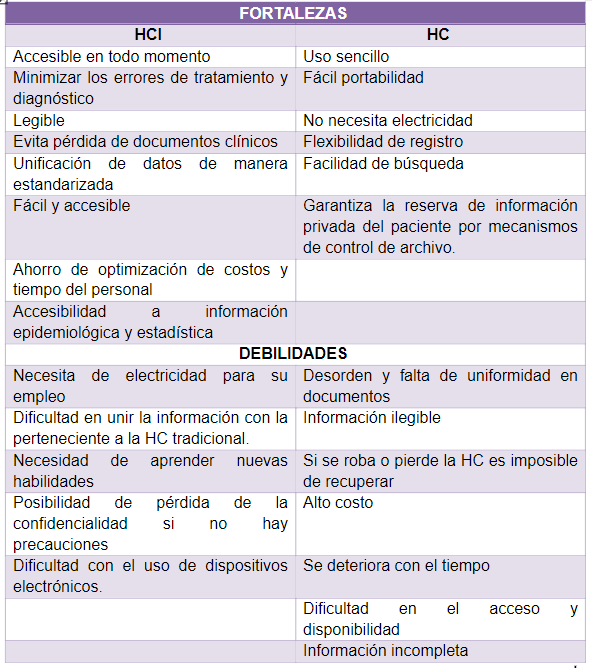
\includegraphics[]{MainMatter/HCIvsHC.PNG}
	\end{figure}
\end{center}


\subsection{Conclusiones}\label{chapter:introduction}


Las ciencias informáticas y bibliográficas han constituido un aporte significativo para el diseño y operación de los sistemas de información del sector sanitario, en especial de la HCI, la cual ha sido aplicada a la medicina veterinaria.

La motivación, y capacitación del personal sanitario, el uso de las herramientas informáticas y de comunicación, y la toma de decisiones basada en evidencias demostrables, se convierten en la piedra angular de los servicios de atención veterinaria.

Por ende, la historia clínica veterinaria constituye un documento único confidencial e individual, en el cual queda plasmado el pronóstico, tratamiento y la evolución del paciente, de ahí la importancia de su correcta confección. 
	

\newpage
\section{Aplicaciones desarrolladas en Cuba en favor del Bienestar Animal}\label{chapter:introduction}

\subsection{Web del Registro Cubano de Mascotas (RCM)}\label{chapter:introduction}


%\begin{figure}[h!]
%\begin{center}
%
\includegraphics[scale=0.4]{Graphics/images/LogodelRegistroCubanodeMascotas.jpg}
%\caption{Logo del Registro Cubano de Mascotas}
%\label{fig:rcm}

%\end{center}
%\end{figure}


Luego de más de 30 años de lucha finalmente Cuba aprueba un Proyecto de Ley sobre protección animal que busca defender los derechos de animales silvestres, de granja y de compañía. Los animales de granja y silvestres tienen derechos y una connotación legal y ética, pero no social. En cambio, los de compañía si pueden y deben entrar en este grupo por su vinculación estrecha al dueño, su familia y el entorno comunitario. Desde esta perspectiva se hace obligatorio que la mascota sea identificada oficialmente y cambiar su estatus de objeto a sujeto. En una reunión efectuada en marzo de 2006 en el Consejo Científico Veterinario de la Habana algunos médicos, técnicos y estudiantes veterinarios abogaron por realizar un estudio para un registro de las mascotas a través de una intranet del Instituto de Medicina Veterinaria. Su objetivo era poder acceder a los datos de las mascotas desde cualquier lugar del país.

Con este enfoque se crea la \textbf{web del Registro Cubano de Mascotas}\brackcite{insReg}, un espacio digital que brinda identificación, respaldo en el cuidado, protección y tenencia responsable de los animales de compañía. Como una de las particularidades se destaca la posibilidad de obtener un documento de identidad, totalmente gratuito; que llevará en él todos los datos de los animales que se inscriben y las de su persona responsable. Este es un proceso sencillo e intuitivo en el que se deben realizar los pasos mostrados a continuación:

\begin{itemize}
\item Acceder a través del teléfono celular o una computadora al sitio www.mascotascuba.com
\item Rellenar los datos solicitados como nombre de la mascota, fecha de su nacimiento, sexo, raza, foto, dirección.
\item Ingresar el correo electrónico o teléfono del tutor de la mascota.
\end{itemize}

Hasta agosto de 2021, estaban oficialmente registrados en la plataforma alrededor de 21 000 animales. De ellos, el $60 \%$ eran perros, $30 \%$ gatos, $7 \%$ aves y un $3 \%$ de roedores, reptiles, equinos, bovinos, porcinos, y otras especies.

\subsection{BACuba}\label{chapter:introduction}

%\begin{figure}[h!]
%\begin{center}
%
\includegraphics[scale=0.09]{Graphics/images/LogodeBienestarAnimalenCuba.png}
%\caption{Logo de Bienestar Animal en Cuba}
%\label{fig:bac}

%\end{center}
%\end{figure}

\textbf{ BACuba}\brackcite{apMov} \brackcite{cubDis} es una aplicación para teléfonos móviles que tiene como fin lograr el bienestar animal y sensibilizar a las personas para la protección de estos seres vivos. Dicha aplicación es una iniciativa de la organización \textbf{Bienestar Animal Cuba}\brackcite{pOBAC}, la mayor red de voluntarios para la protección animal. Fue lanzada desde el pasado 19 de enero de 2022, y se basa en el principio que rige la organización: rescatar animales abandonados y brindarles todos los cuidados. También buscan promover campañas, actividades, ferias y spots para garantizar el bienestar animal. Esta novedosa aplicación posee varias utilidades separadas en varias secciones:

\begin{itemize}
\item \textbf {Adoptar}: En este panel se muestran todos los datos (nombre, edad, sexo, raza) y con una foto incluida de los animales que están en adopción, ya sea perros, gatos u otros.
\item \textbf{ Reportes}: Esta es una de las secciones más humanas, ya que los usuarios podrán reportar desapariciones de mascotas, acciones de maltrato animal, atropellos, abandonos, animales en estado de vulnerabilidad. Pueden hacerlo desde cualquier parte del país y con estas denuncias los voluntarios de las distintas redes de ayuda animal o cualquier persona sensibilizada tomarán cartas en el asunto.
\item \textbf{Cuidados}: En este apartado se brindan informaciones de mucha ayuda para los dueños de mascotas y que son útiles para todas las provincias y municipios del país. Por ejemplo, una lista con direcciones y teléfonos de las principales clínicas veterinarias, tiendas de accesorios y medicinas para sus mascotas, y algunos artículos de interés para aumentar la cultura del cuidado animal.
\item \textbf{Noticias}: Aquí te podrás enterar de eventos relevantes como ferias de adopciones a lo largo de toda Cuba, donaciones y otras actividades en las que quizás te interese participar.
\item \textbf{Mis Mascotas}: En este apartado podrás registrar a tus animales con sus nombres, fecha de nacimiento, y todos los datos de su carnet de identidad, en el caso de poseer uno. En esta base de datos podrás incluir, además, un registro con los días de vacunación y desparasitación, a modo de recordatorio.
\end{itemize}

Información general de BACuba:


\begin{itemize}
\item Funciona con los datos móviles activados o por medio de servicio Wifi.
\item Está diseñada únicamente para dispositivos móviles, con un tamaño de 12.60 MB y requiere una versión de Android 5.0 o versiones superiores.
\item Es útil para cualquier lugar del país.
\item Puede ser descargada, libre de costo, de la plataforma APKLIS.
\item Tiene un diseño sencillo pero atractivo, y cumple con su función de informar, orientar, educar y ayudar en cuanto a materia de protección animal.
\end{itemize}

\section{Aplicaciones móviles que gestionan Historias Clínicas Veterinarias}\label{chapter:introduction}

\subsection{Dog Health}\label{chapter:introduction}

%\begin{figure}[h!]
%\begin{center}
%
\includegraphics[scale=0.12]{Graphics/images/LogodeDogHealth.png}
%\caption{Logo de Dog Health}
%\label{fig:dh}

%\end{center}
%\end{figure}


\textbf{Dog Health}\brackcite{dogHe} es una aplicación totalmente gratuita para móviles y tablets, fue creada por un comunicador italiano, por lo que está solo disponible en el idioma inglés. Creada para llevar el registro veterinario de nuestras mascotas en Android. Dentro de sus principales prestaciones se encuentran:

\begin{itemize}


\item	Guardar los datos personales de las mascotas como su nombre, peso, fecha de nacimiento, número de chip, entre otros.
\item	Hacer un seguimiento de anteriores visitas al veterinario.
\item	Administrar a los veterinarios.
\item	Hacer un seguimiento de las vacunas.
\item	Recordatorios de citas y visitas.
\item	Memorizar todas las administraciones de medicamentos realizadas y por realizar.
\item Buscar y contactar con el veterinario más cercano.
\item	Añadir múltiples mascotas.
\item	Realizar backups y restaurarlos.
\item	Guardar la evolución del peso y altura de las mascotas de forma continuada.

\end{itemize}


\subsection{Pet Soft}\label{chapter:introduction}

%\begin{figure}[h!]
%\begin{center}
%
\includegraphics[scale=0.5]{Graphics/images/LogodePetSoft.png}
%\caption{Logo de Pet Soft}
%\label{fig:dh}

%\end{center}
%\end{figure}


\textbf{ Pet Soft}\brackcite{sofVet} \brackcite{petSo} es una plataforma para veterinarias y dueños de mascotas creada para almacenar y gestionar agendamientos con todo lo relacionado del paciente estableciendo citas, vacunas y todo tipo de información detallada con el fin de contar con un completo historial médico que le permita no solo al profesional veterinario, sino a los dueños de las mascotas acceder de manera segura a la información completa del animal. Esta plataforma es completamente web y la aplicación se puede descargar desde cualquier dispositivo con sistema operativo Android o IOS.

Como ventaja para el usuario sea médico o dueño de la mascota conseguirá descargar la aplicación de forma intuitiva donde podrá ingresar toda la información requerida y vital para los pacientes. Su fortaleza radica en la fácil visualización y datos de carga que aseguran una experiencia agradable para sus usuarios. Con la implementación del software los usuarios pueden gestionar de forma segura y sencilla todo lo relacionado con las mascotas y acceder a la ubicación de la red más completa de veterinarias. La información de cada mascota, se alberga en la web, de modo que, en cada centro veterinario, se podrá descargar, sin necesidad de que se tengan que volver a registrar los datos en el sistema. Dentro de sus principales beneficios se encuentran:

Beneficios para veterinarias:
\begin{itemize}


\item	Consultas y servicios: crear consultas y servicios; todo bajo control del software.
\item	Tarifas y bonos: manejar tus propias tarifas, generar bonos promocionales.
\item	Citas y alarmas: notificaciones para las citas programadas o crear una directamente.
\item	Veterinarias en red: consultar la historia clínica de la mascota si ha estado en otra veterinaria.
\item	Médicos veterinarios: crear usuarios especializados para tu veterinaria.

\end{itemize}

Beneficios para tu mascota:
\begin{itemize}


\item	Datos básicos: registrar todas las mascotas.
\item	Historia clínica: llevar el historial de las consultas de tus mascotas directamente de las veterinarias.
\item	Citas: notificaciones para las citas programadas o crear una directamente.
\item	Veterinarias: un mapa para buscar la veterinaria más cercana.
\item	Carné: llevar en la app el carnet de vacunación de tus mascotas.
\end{itemize}


\subsection{Petmeddata}\label{chapter:introduction}


\textbf{Petmeddata} \brackcite{petMed}\brackcite{petMed2} es un sistema electrónico seguro para almacenar el historial médico de todas las mascotas en un solo sitio. Creado en Finlandia a finales de 2018, facilita el tratamiento integral de los animales ya que muestra instrucciones de alta, medicamentos y valores de laboratorio en orden cronológico. Los problemas de seguridad se han considerado cuidadosamente. El dueño del animal decide quién puede ver la información de la mascota. Si el propietario comparte el perfil con una nueva clínica, esta puede ver las secciones más importantes del historial clínico en el historial del paciente. El personal de la clínica también ve las entradas, textos e imágenes del propietario. Nadie puede ver el precio y la información de pago, ni las notas de la clínica de animales. El nombre del animal o el microchip nunca aparecerán en ninguna parte. Para dueños de animales y clínicas de animales, el sistema es gratuito. A los socios se les cobra una tarifa por prestar sus servicios en el sistema.
“Al utilizar $Petmeddata$, el dueño siempre tiene consigo el historial médico de la mascota, incluso si va a una nueva clínica. Y el veterinario podrá leer en un formato fácil de leer lo que se le ha hecho al animal en el pasado. No hay necesidad de llevar papeles escritos a mano o impresos”, dice la Gerente de Proyecto Eva Kaisti.

Entre sus principales características se encuentran:
\begin{itemize}


\item	Fácil acceso online a todos los datos sanitarios de las mascotas; crea el perfil médico para cada uno de tus animales y contrólalos desde un solo sitio
\item	Veterinarios y otros expertos envían los datos médicos oficiales al perfil del animal.
\item	Posibilidad de añadir tus propios documentos y notas.
\item	Funciona por conexión a internet desde un teléfono móvil, tablet u ordenador.
\item	Sitio seguro; no almacena información personal tuya, sólo la información médica de tus mascotas.
\item	Posibilidad de compartir el perfil de las mascotas con un profesional del cuidado de los animales, como un veterinario, un amigo, guardería para mascotas, etc.
\end{itemize}


\subsection{VitusVet}\label{chapter:introduction}

\textbf{VitusVet} \brackcite{vitPet} es un $software$ de administración de prácticas veterinarias que permite a veterinarios y clínicas manejar el flujo de trabajo, comunicaciones con clientes, pagos, historias clínicas, horarios de consultas, entre otros. Permite el envío y recibimiento de texto, imágenes y actualizaciones en tiempo real.

Usando aplicaciones móviles de $VitusVet$ múltiples veterinarios pueden compartir historias clínicas de mascotas con clientes y hacer recordatorios sobre encuentros futuros. La plataforma $VitusPay$ permite a los dueños de mascota realizar pagos mensuales a través de tarjetas de crédito. Los clientes pueden pedir consultas con los veterinarios a través de mensajes de texto, emails, plataformas de redes sociales y aplicaciones móviles. El $software$ permite a veterinarios configurar y automatizar respuestas basándose en el personal disponible, horario de trabajo, días feriados y enviar recordatorios a través de postales personalizadas. 





\subsection{Conclusiones de las aplicaciones presentadas}\label{chapter:introduction}

En esta sección se analizaron aplicaciones con similitudes a la que se plantea como finalidad en este documento. Todo esto con el objetivo de adoptar las ideas de la competencia o mejorarlas dependiendo del caso, sobre este tema se puede afirmar lo siguiente:

\begin{enumerate}


\item	En general las herramientas en esta sección permiten la creación y el manejo de las historias clínicas digitales para nuestras mascotas, pero como se observó en cada caso estas no brindan la posibilidad para exportar de manera offline\footnote{La tranferencia de datos offline en $Android$ refiere a una forma de enviar datos de forma inalámbrica sin necesidad de conexión a Internet, existen varias tecnologías que permiten este tipo de transferencia como $Wifi$ $Direct$, $Bluetooth$, $SIP$, etc.} \brackcite{offDT} los datos de las mascotas que queramos compartir con otro usuario. Entre los objetivos de este trabajo está la mejora de este aspecto.



\item	Pocas de estas aplicaciones permiten al usuario consultar los datos de sus mascotas sin la necesidad de una conexión a Internet, aspecto que goza de gran peso entre los principales objetivos de este trabajo.
\item	Las herramientas para el manejo de las historias clínicas desde un dispositivo móvil, permiten a los usuarios ya sean médicos veterinarios o dueños y encargados de las mascotas acceder de manera sencilla y segura a toda la información referente al estado de salud, seguimiento, y cuidado del animal.
\item	Luego de analizar las aplicaciones anteriores se concluye como necesario el diseño de una aplicación que si cumpla con los requerimientos expuestos en este documento, porque en general estas aplicaciones no permiten el trabajo con historias clínicas animales de manera offline, aspecto de vital importancia debido a las limitaciones de la conexión a Internet que presenta nuestro país.
\end{enumerate}

\section{Tecnologías para el desarrollo de aplicaciones móviles}\label{chapter:introduction}

\subsection{Programación Nativa de Android : Java y Kotlin}\label{chapter:introduction}

El desarrollo de aplicaciones nativas es una opción increíble para ofrecer a los usuarios la experiencia más satisfactoria en términos de la sensación y la apariencia de su aplicación. 



\subsection{React Native}\label{chapter:introduction}



%\begin{figure}[h!]
%\begin{center}
%
\includegraphics[scale=0.5]{Graphics/images/LogodeReactNative.jpg}
%\caption{Logo de React Native}
%\label{fig:dh}

%\end{center}
%\end{figure}


\textbf{React Native}\brackcite{reaNative} es un framework que permite construir aplicaciones móviles nativas, para iOS y Android (así como también para Android TV, macOS, tvOS, Windows y UWP\footnote{Universal Windows Platform}  , aunque nos enfocaremos en los dos gigantes de la telefonía móvil), utilizando solamente JavaScript y React.

Utiliza el mismo diseño que React.js, permitiendo usar elementos de interfaz de usuario móvil. A pesar de que React.js y React Native usen la misma estructura de código, no sirven para lo mismo, mientras React.js es utilizado para hacer páginas web y trabaja con elementos del virtual DOM, por el otro lado React Native utiliza elementos nativos de interfaz de usuario de Android y iOS (entre otras) para crear aplicaciones para ambas plataformas.

Habiendo mencionado la UI, React Native usa el mismo paradigma fundamental de construcción de bloques para la interfaz de usuario que las aplicaciones nativas puras de Android e iOS (a los que React Native denomina Componentes), pero gestiona la interacción entre los mismos utilizando las capacidades de JavaScript y React.

Similar a React para web, en este caso las aplicaciones están escritas usando una mezcla de JavaScript y marcado XML, conocido como JSX\footnote{JavaScript Syntax Extension y ocasionalmente mencionado como JavaScript XML} . Luego, detrás del telón, el conocido \textbf{bridge} o puente de React Native invoca las APIs de renderizado nativas en Objective-C (para iOS) o Java (para Android). React Native también expone interfaces JavaScript para las API de la plataforma, por lo que sus aplicaciones pueden acceder a sensores y funciones de la plataforma como la cámara del teléfono o la ubicación del usuario.

React Native surgido por la necesidad de una solución nativa para los problemas que presentaba el uso de HTML5 en la versión móvil de Facebook, que resultó en una aplicación inestable y con poca fluidez. La idea surge a partir de Jordan Walke, ingeniero de software de Facebook, que encontró una forma de generar elementos de interfaz de usuario para iOS a partir de un hilo de JavaScript en segundo plano, lo que sentó las bases de lo que sería React para la web. Esto unido al interés de la compañía llevó a que meses más tarde Facebook lanzara la primera versión de React.js, y Christopher Chedeau\footnote{También conocido como Vjeux, es un ingeniero front-end en Facebook que se graduó de EPITA (la primera escuela de ingenieros especializada en informática de París)} , durante una charla técnica explicara, que Facebook ya estaba usando React Native en producción para su aplicación de grupo y su aplicación de administrador de anuncios.

Ventajas
\begin{enumerate}

\item	Traduce su marcado a elementos de UI nativos reales, además, React funciona por separado del hilo principal de la interfaz de usuario, por lo que su aplicación puede mantener un alto rendimiento sin sacrificar la capacidad.
\item	Para los desarrolladores acostumbrados a trabajar en la Web con React.js, significa que pueden desarrollar aplicaciones móviles con el rendimiento y la apariencia de una aplicación nativa, mientras usan herramientas familiares.
\item	Una comunidad sólida, hay miles de colaboradores que actualizan constantemente la biblioteca.
\item	Permite optimizar las aplicaciones nativas por separado escribiendo código específico de cada plataforma y usándolo desde JavaScript.
\item	Mejora la experiencia de desarrollo gracias a su Hot Reload o recarga en caliente, que permite a los desarrolladores visualizar cambios efectuados en la aplicación de inmediato, sin necesidad de re-compilar todo el proyecto.
\item	Alta fiabilidad al estar respaldada por Facebook, siendo usada como herramienta de desarrollo por grandes empresas como Instagram, Microsoft, Pinterest y Walmart.
\end{enumerate}

Desventajas
\begin{enumerate}



\item	La navegación integrada en React Native no es perfecta y no es comparable a la navegación nativa.
\item	Tiene dificultades para crear transiciones y animaciones complejas.
\item	Debido a que React Native es una abstracción sobre las API existentes de Android y iOS, usualmente cuando hay nuevas versiones puede ser que esa funcionalidad tarde un poco en llegar a la plataforma aunque siempre llega.
\item La documentación es deficiente para algunos casos, producto a la misma velocidad con que se realizan actualizaciones, muchos colaboradores no consideran necesaria su documentación sobre la marcha.
\end{enumerate}



\subsection{Xamarin}\label{chapter:introduction}

\textbf{Xamarin} \brackcite{xama} es un kit de herramientas de desarrollo de aplicaciones multiplataforma que nos permite producir aplicaciones nativas de $Android$, $iOS$, $tvOS$, $watchOS$, $macOS$ y $Windows$ con $UI$ unificadas, siendo parte en la actualidad de la plataforma de desarrollo $.NET$  \footnote{$.NET$ es una plataforma de desarrollo compuesta por herramientas, lenguajes de programación y bibliotecas para crear muchos tipos diferentes de aplicaciones.} \brackcite{net}. Fue en sus inicios construida como herramienta por los desarrolladores de Mono \footnote{Mono es una plataforma de desarrollo de código abierto basada en .NET Framework, dirigida por Miguel de Icaza y presentada por primera vez en 2001}  y siendo fundada como compañía homónima el 16 de mayo del 2011, para ser adquirida en el 2016 por Microsoft.
Fue para cuando Microsoft adaptó el $Kit$ de Desarrollo de Software ($SDK$) \footnote{Un $kit$ de desarrollo de software ($SDK$) es un conjunto de herramientas proporcionado usualmente por el fabricante de una plataforma de $hardware$, un sistema operativo o un lenguaje de programación.} de Xamarin a sus políticas de código abierto como hizo con $.NET$, que se convirtió en parte del entorno de desarrollo integrado de Xamarin Visual Studio lo cual le dio gran aceptación dentro del mundo de desarrolladores $.NET$.

Xamarin requiere de un solo lenguaje para desarrollar aplicaciones para las distintas plataformas, ese lenguaje es $C\#$. Los proyectos con Xamarin compilan de forma nativa, lo que lo convierte en una opción para crear aplicaciones con un alto rendimiento y con un aspecto nativo. Estas aplicaciones a menudo se comparan con las nativas para las plataformas de desarrollo móvil $iOS$ y $Android$ en términos de rendimiento y experiencia del usuario. En las aplicaciones desarrolladas con Xamarin el código relacionado a la lógica de negocios, el manejo de la Base de datos y el acceso a la red puede ser compartido entre todas las plataformas y a su vez permitir desarrollar una capa de interfaz de usuario diferenciada para cada plataforma, permitiendo que las aplicaciones compiladas de esta manera, se vean de forma nativa.
Con Xamarin se puede desarrollar en $Windows$ o $Mac$ y compilarse en paquetes de aplicaciones nativas, como un archivo $.apk$ en Android o uno $.ipa$ en $iOS$.

Ventajas:

\begin{itemize}


\item	Se encuentra embebido en el ecosistema de $.NET$ $Framework$, con todas las facilidades de Visual Studio concentrando todas las herramientas que eran accesibles desde Xamarin Studio junto con todo lo necesario para el trabajo con $C\#$ y más, de forma gratuita.
\item	Xamarin tiene una documentación bien estructurada que incluye casos, fragmentos y tutoriales paso a paso.
\item	El desarrollo multiplataforma de Xamarin requiere aproximadamente 1,5 veces menos tiempo (y dinero) que el desarrollo de un proyecto nativo independiente para cada plataforma.
\item	Las aplicaciones que se construyen en Xamarin nos darán un mejor rendimiento y mejorarán constantemente para que coincidan con los estándares de desarrollo nativo. A diferencia de las soluciones híbridas tradicionales, basadas en las tecnologías web, una aplicación multiplataforma desarrollada con Xamarin puede clasificarse como nativa en términos de rendimiento.
\item	Permite crear experiencias visuales completamente nativas. Incluso por herramientas asociadas como Xamarin.Forms convierte los componentes de la interfaz de usuario de la aplicación en elementos propios de la plataforma en tiempo de ejecución. Esta última, disminuyendo el tiempo de desarrollo sustancialmente pero con sacrificios leves en el rendimiento debido a la capa de abstracción adicional.
\item	Xamarin $SDK$, que incluye tiempo de ejecución, bibliotecas y herramientas de línea de comandos, pasa a ser de código abierto, estando disponible para todos bajo la licencia $MIT$  como parte de Visual Studio a partir de febrero de 2016, lo que acelera el crecimiento de la plataforma.

\end{itemize}


Desventajas:

\begin{itemize}


\item	Dependiendo del proyecto las aplicaciones desarrolladas por esta tecnología tienden a ocupar más espacio en memoria. Para ilustrar lo anterior una aplicación de Hola Mundo desarrollada con Xamarin para Android puede alcanzar los $16$ MB, en su estado puro, sin paquetes adicionales, mientras que la desarrollada de forma nativa puede ser menor a los $3$ MB.
\item	Puede haber trabas al integrar recursos de terceros con la aplicación en Xamarin. Aunque la mayoría de las herramientas y bibliotecas ofrecen soporte completo para tecnologías nativas, es posible que un proveedor no brinde soporte de Xamarin. Siempre existe la posibilidad de que necesite una capacidad o integración específica dentro de su aplicación que no sea proporcionada por la plataforma o su tienda de componentes.
\item	A pesar del tiempo en el mercado Xamarin.IOS, Xamarin.Android e incluso Xamarin.Forms se le presentan quejas sobre estabilidad, errores y fallas. Principalmente Xamarin.Forms que es más usado por su posibilidad de ahorrar tiempo creando prototipos y aprovechar al máximo el código compartido. Algunos desarrolladores se muestran inconformes afirmando que, en lugar de ahorrar tiempo con el uso compartido de código, puede terminar empleando más tiempo resolviendo problemas.
\end{itemize}																																																																																																																																																																																																																																																																																					


\subsection{Flutter}\label{chapter:introduction}


%\begin{figure}[h!]
%\begin{center}
%
\includegraphics[scale=0.5]{Graphics/images/LogodeFlutter.jpg}
%\caption{Logo de Flutter}
%\label{fig:dh}

%\end{center}
%\end{figure}


\textbf{Flutter} \brackcite{flu} es un conjunto de herramientas de interfaz de usuario multiplataforma que está diseñado para permitir la reutilización de código en sistemas operativos como iOS y Android, al mismo tiempo que permite que las aplicaciones interactúen directamente con los servicios de la plataforma subyacente. El objetivo es permitir que los desarrolladores entreguen aplicaciones de alto rendimiento que se sientan naturales en diferentes plataformas, adoptando las diferencias donde existen mientras comparten la mayor cantidad de códigos posibles.

Se trata de un conjunto de herramientas de Interfaz de usuario portátiles que fueron creados por Google. Este es un framework bastante nuevo, presentado por primera vez en 2015 \brackcite{dart}, que pasó algunos años perfeccionándose en las versiones. La primera versión estable, Flutter 1.0, fue lanzado el 4 de diciembre de 2018. En el último año, ha experimentado un crecimiento muy grande en cuanto a su popularidad, esto debido a su velocidad de desarrollo, experiencia nativa y eficiente renderización de la interface. Sería para el 3 de marzo de 2021, en el evento virtual llamado Flutter Engage, que Google lanza Flutter 2, el que fuese su cambio oficial más grande, dejando de ser solo un SDK para aplicaciones móviles, convirtiéndose en un framework para el desarrollo multiplataforma incluyendo además de Android y iOS, a Windows, Linux, MacOS y Web. Como cambios en esta versión incluyendo null safety \footnote{Cuando se opta por la seguridad nula, los tipos de su código no admiten nulos de forma predeterminada, lo que significa que las variables no pueden contener nulos a menos que usted lo indique explícitamente}, uno de los más emblemáticos, característica opcional al momento de crear un nuevo proyecto (siendo también posible migrar proyectos ya existentes a la nueva forma).

Flutter es un producto de código abierto, desarrollado en $C$, $C++$, Dart y Skia Graphics Engine, este último una biblioteca gráfica compacta, que también fue adquirida por Google. El lenguaje de programación estándar utilizado por Flutter es Dart, para quien no sabe, Dart es un lenguaje de propósito general un poco más antiguo que Flutter. Este fue creado en 2011 por Google para sustituir JavaScript, cuya tentativa no fue del todo exitosa, para convertirse en lo que conocemos hoy, con un lenguaje muy versátil pudiendo ser utilizado en varios entornos, con herramientas integradas que facilitan el desarrollo y teniendo a Flutter como principal objetivo del lenguaje actualmente.

Ventajas
\begin{enumerate}

\item	La representación en todas las plataformas es la misma, sin necesidad de implementar código específico para cada plataforma, independientemente de si se ejecuta en Android o diferentes versiones de iOS.
\item	Con Flutter, los desarrolladores ya no tienen que lidiar con un largo tiempo en recargar su aplicación, gracias al ya mencionado Hot Reload. Pero al contrario de estos otros frameworks, la mayoría de los cambios en la interfaz de usuario se aplican mientras el desarrollador todavía está trabajando en el código, de forma instantánea.
\item	Hace que sea más fácil no solo ver la interfaz de usuario, sino también crearla (diseñar un tema en una aplicación nativa de Android puede ser un desafío, con Flutter, crear un tema es mucho más sencillo). La compatibilidad con temas incorporada hace que el diseño de todos los aspectos de la interfaz de usuario sea más rápido y fácil para los desarrolladores.
\item	La documentación oficial es excelente y completa, paquetes bien documentados, contando con un ritmo alto de actualizaciones y una comunidad numerosa, con muchas conferencias y eventos anualmente.
\item	El lenguaje de programación Dart es muy similar a Java / Kotlin (Android), lo que facilita el aprendizaje para los desarrolladores que provienen del desarrollo móvil nativo.
\item	Ha conseguido generar confianza y seguridad en los profesionales que trabajan con él, por el hecho de que una empresa como Google está detrás, además del auge que está experimentando Flutter en los últimos meses, las actualizaciones de las librerías y los widgets, así como el mantenimiento, de manera constante.

\end{enumerate}

Desventajas
\begin{enumerate}


\item	Al ser un framework bastante reciente con 3 años y medio (para el momento de este documento), implica que el desconocimiento y la experiencia que se tiene en su uso es mucho menor que con otros sistemas de desarrollo.
\item	Presenta un mayor tamaño de las aplicaciones en el caso de iOS. En diciembre de 2018, se midió el tamaño de descarga de una aplicación Flutter mínima Hello World, arrojando como resultados, un peso de 4,06 MB para el caso de Android y 10,8 MB para el caso de iOS, el IPA  es mayor que el APK principalmente porque Apple encripta binarios dentro del IPA\footnote{Es una extensión de archivo por sus siglas en inglés IPhone Application, referente al software que se puede instalar en la plataforma del sistema iOS y MacOS}, haciendo la compresión menos eficiente \brackcite{appDev}.
\item	Pocas bibliotecas. A pesar de tener muchas bibliotecas nativas de Flutter que funcionan muy bien, cuando se trata de bibliotecas de terceros, las cosas no se ven tan bien. La cantidad de soluciones en Flutter es menor que la cantidad de paquetes disponibles para desarrollo nativo o React Native.
\end{enumerate}

\subsection{Conclusiones sobre las plataformas mostradas}\label{chapter:introduction}

La comparación está bastante equiparada, para el caso de React Native cuenta con una amplia comunidad, gran número de paquetes y posee un buen rendimiento, pero un motor gráfico aún deficiente y carece de fluidez para las animaciones más simples. Mientras Flutter a pesar de poseer una comunidad aún pequeña en comparación con React Native o Xamarin, es cooperativa y esta creciendo en una magnitud superior a la de ambas.

Flutter llega para suplir, con creces, las deficiencias de React Native respecto al apartado gráfico y los problemas de estabilidad que padece Xamarin, con una excelente documentación y un lenguaje de programación que aunque no es tan conocido como JavaScript, es muy poderoso y cuenta con una sintaxis similar a la de Java y $C\#$. Con aplicaciones optimizadas para ocupar menos espacio, donde a pesar no ser rivales para las desarrolladas de forma nativa, supera a la competencia en ese aspecto.

Luego de todo lo expuesto, sumado a la experiencia previa que se posee en el uso de \textbf{Flutter} para el desarrollo multiplataforma,\textbf{ fue seleccionado para implementar la aplicación} que concluirá este trabajo.

\section{Tecnologías para el desarrollo de base de datos}\label{chapter:introduction}





\subsection{Bases de Datos para Android}\label{chapter:introduction}

Generalmente las bases de datos se manejan en el lado del servidor o en la nube y los dispositivos móviles solo se comunican con ellos a través de la red. Esto implica que la aplicación móvil necesite una conexión de red activa y bastante rápida para acceder a sus datos. Sin embargo, para hacer que las aplicaciones sean más receptivas y menos dependientes de la conectividad de la red, la tendencia del uso fuera de línea o la menor dependencia de la red está ganando popularidad.

Hoy en día, las aplicaciones mantienen la base de datos localmente o hacen una copia en la nube y en el dispositivo local y se sincronizan con ella una vez al día o cada vez que hay una conectividad de red. Esto ayuda a crear aplicaciones más rápidas y receptivas que son funcionales incluso cuando no hay conectividad a Internet o es limitada.

Las bases de datos para Android deben ser:
\begin{itemize}


\item	Ligeras ya que el almacenamiento es limitado en dispositivos móviles.
\item	Sin requisito de servidor.
\item	En una forma de biblioteca con ninguna o muy limitada dependencia (incrustable\footnote{Las bases de datos incrustadas son bibliotecas livianas y autónomas sin componentes de servidor, sin necesidad de administración.} ) para que se pueda usar cuando sea necesario.
\item	Rápidas y seguras.
\item	Fácil de manejar mediante código y opción para hacerlas privadas o compartidas con otras aplicaciones.
\item	Requerir poca memoria y consumo de energía.
\end{itemize}

Existen muchas bases de datos para Android y móviles en el mercado, pero no todas satisfacen todos los requisitos mencionados en este Trabajo. Vamos a discutir algunas de las bases de datos más populares para aplicaciones móviles y tratar de resaltar sus características, pros y contras.

\subsection{Berkeley DB}\label{chapter:introduction}



%\begin{figure}[h!]
%\begin{center}
%
\includegraphics[scale=0.5]{Graphics/images/LogodeBerkeleyDB.jpg}
%\caption{Logo de BerkeleyDB}
%\label{fig:bdb}

%\end{center}
%\end{figure}


\textbf{ Berkeley DB (BDB)}\brackcite{orBer} es una biblioteca de software destinada a proporcionar una base de datos integrada de alto rendimiento para datos clave/valor. Berkeley DB está escrito en C con enlaces API para C++ , $C\#$ , Java , Perl , PHP , Python , Ruby , Smalltalk , Tcl y muchos otros lenguajes de programación. BDB almacena pares de clave/datos arbitrarios como matrices de bytes y admite varios elementos de datos para una sola clave. Berkeley DB no es una base de datos relacional, aunque tiene funciones de base de datos avanzadas que incluyen transacciones de base de datos, control de concurrencia multiversión y registro de escritura anticipada.

Fue desarrollado y respaldado comercialmente por Sleepycat Software de 1996 a 2006. Sleepycat Software fue adquirido por Oracle Corporation en febrero de 2006, que continúa desarrollando y vendiendo la biblioteca C Berkeley DB. Desde su lanzamiento inicial, Berkeley DB ha pasado por varias versiones. Cada ciclo de lanzamiento importante ha introducido una sola característica principal nueva que generalmente se superpone a las características anteriores para agregar funcionalidad al producto. La evolución a veces ha llevado a cambios menores en la API o cambios en el formato de registro, pero muy rara vez han cambiado los formatos de la base de datos. Berkeley DB HA admite actualizaciones en línea de una versión a la siguiente al mantener la capacidad de leer y aplicar los registros de la versión anterior.

Entre sus principales características se encuentran: 
\begin{itemize}


\item	Los datos se almacenan en el formato nativo del lenguaje de programación.
\item	No tiene modo cliente-servidor.
\item	Caché configurable para modificar el rendimiento.
\item	Permite crear bloqueos de forma detallada. Esto es especialmente útil para trabajos concurrentes sobre la base de datos de forma que se bloquea una página de registros durante una transacción para evitar que se modifiquen hasta que termine, pero permitiendo actuar sobre el resto de páginas.
\item	Posibilidad de realizar copias de seguridad y replicación.
\item	Transacciones y recuperación ante errores ACID. Esto es configurable de forma que se puede ir relajando en función de la aplicación.
\item	Es compatible con algunas interfaces históricas para bases de datos en UNIX.
\item	Permite utilizar la característica de snapshots para poder efectuar varias transacciones sobre los mismos registros de manera simultánea.
\item	No soporta SQL ni esquemas. A pesar de esto tiene un tamaño superior al de otras alternativas incrustadas (ocupa casi el doble que SQLite).
\end{itemize}


\subsection{Couchbase Lite}\label{chapter:introduction}


\textbf{Couchbase Lite}\brackcite{cblite} es un motor de base de datos sincronizable, liviano, orientado a documentos ($NoSQL$) integrado. Al estilo de Couchbase Server maneja documentos $JSON$ y tiene el mismo mapa/reducción que este en una edición pequeña. Está escrito en $Objective-C$ y $C++$ y se requiere $Xcode$ $7$ o posterior para construirlo. Couchbase Lite compila de forma nativa para $iOS$, $Android$, $Mac OS$ y $.NET$. Medio megabyte optimizado, para un inicio rápido y una experiencia de usuario ágil en dispositivos conectados ocasionalmente cuando los datos importan.

Entre sus principales características se encuentran: 
\begin{itemize}


\item	Es integrado; el motor de la base de datos es una biblioteca vinculada a la aplicación, no un proceso de servidor independiente.
\item	Tamaño de código pequeño, actualmente menos de $600$ kbytes. 
\item	Bajo uso de memoria con conjuntos de datos móviles típicos. La expectativa es que la cantidad de documentos no sea enorme, aunque puede haber archivos adjuntos multimedia considerables.
\item	Al igual que Couchbase Server, almacena registros en formato $JSON$ flexible en lugar de requerir esquemas predefinidos o normalización.
\item	Los registros/documentos pueden tener archivos adjuntos binarios de tamaño arbitrario, como contenido multimedia.
\item	El formato de datos de su aplicación puede evolucionar con el tiempo sin necesidad de migraciones explícitas.
\item	Mapear/reducir el indexado permite búsquedas rápidas sin necesidad de utilizar lenguajes de consulta especiales.
\item	El motor de sincronización admite conexiones de red intermitentes y poco fiables.
\item	Las $API$ nativas son $Objective-C$ ($iOS$, $tvOS$, $Mac$), $Java$ ($Android$) y $C\#$ ($.NET$, Xamarin); pero un adaptador $API$ $REST$ interno opcional permite llamarlo desde otros lenguajes como JavaScript, para usar en aplicaciones creadas con PhoneGap/Cordova o Titanium.

\end{itemize}

\subsection{SQLite}\label{chapter:introduction}




\textbf{SQLite} \brackcite{sqli} es una biblioteca en proceso que implementa un motor de base de datos SQL transaccional autónomo, sin servidor y sin configuración. El código de SQLite es de dominio público y, por lo tanto, es de uso gratuito para cualquier propósito, comercial o privado. SQLite es la base de datos más implementada en el mundo con más aplicaciones de las que podemos contar, incluidos varios proyectos de alto perfil. A diferencia de la mayoría de las otras bases de datos SQL, SQLite no tiene un proceso de servidor separado. SQLite lee y escribe directamente en archivos de disco ordinarios. Una base de datos SQL completa con varias tablas, índices, $triggers $(disparadores) y vistas está contenida en un solo archivo de disco. El formato de archivo de la base de datos es multiplataforma: puede copiar libremente una base de datos entre sistemas de 32 y 64 bits o entre arquitecturas big-endian y little-endian. Estas características hacen de SQLite una opción popular como formato de archivo de aplicación. 

El código base de SQLite cuenta con el respaldo de un equipo internacional de desarrolladores que trabajan en SQLite a tiempo completo. Los desarrolladores continúan expandiendo las capacidades de SQLite y mejorando su confiabilidad y rendimiento mientras mantienen la compatibilidad con las especificaciones de interfaz publicadas, la sintaxis SQL y el formato de archivo de la base de datos. El código fuente es absolutamente gratuito para cualquiera que lo desee, pero también hay soporte profesional disponible. El proyecto SQLite se inició el 9 de mayo del 2000. El futuro siempre es difícil de predecir, pero la intención de los desarrolladores es admitir SQLite hasta el año 2050. Las decisiones de diseño se toman con ese objetivo en mente.

Entre sus principales características se encuentran:
\begin{itemize}

\item	Las transacciones son atómicas, consistentes, aisladas y duraderas (ACID)\footnote{$ACID$ es un conjunto de propiedades de las transacciones de base de datos que tienen como propósito garantizar la validez de los datos a pesar de posibles errores, fallos de energía u otros problemas que pueden surgir} incluso después de fallas del sistema y fallas de energía.
\item	No se necesita configuración ni administración.
\item	Implementación completa de SQL con capacidades avanzadas como índices parciales, índices en expresiones, JSON, expresiones de tablas comunes y funciones de ventana.
\item	Una base de datos completa se almacena en un único archivo de disco multiplataforma. Ideal para usar como formato de archivo de aplicación.
\item	Admite bases de datos del tamaño de un terabyte y cadenas y blobs del tamaño de un gigabyte.
\item	API simple y fácil de usar.
\item	Rápido, en algunos casos, SQLite es más rápido que la E/S directa del sistema de archivos.
\item	Código fuente bien comentado con una cobertura de prueba de rama del 100 %.
\item	Disponible como un solo archivo de código fuente ANSI-C que es fácil de compilar y, por lo tanto, fácil de agregar a un proyecto más grande.
\item	Autónomo; sin dependencias externas.
\item	Multiplataforma: Android, BSD, iOS, Linux, Mac, Solaris, VxWorks y Windows (Win32, WinCE, WinRT) son compatibles desde el primer momento. Fácil de portar a otros sistemas.
\item	Las fuentes son de dominio público. Uso para cualquier propósito.
\end{itemize}

\subsection{Conclusiones sobre las bibliotecas mostradas}\label{chapter:introduction}

Luego de analizar las características que presentan las bibliotecas antes mencionadas para la creación y el manejo de las bases de datos. Así cómo sus ventajas y desventajas propias de las bases de datos relacionales y no relacionales, y las características que deben tener las bases de datos para Android, \textbf{se decidió por SQLite}.

$SQLite$ permite que el desarrollo sea más simple. Los paquetes android.database y android.database.sqlite ofrecen una alternativa de mayor rendimiento donde la compatibilidad de la fuente no representa mayor problema, aprovechando los recursos. Es ideal para consultar y almacenar datos de forma estructurada. La aplicación solo tiene que cargar tantos datos como necesite, en lugar de leer todo el archivo de la aplicación y mantener un análisis completo en la memoria, por ende, el tiempo de inicio y el consumo de memoria se reducen. El contenido se actualiza de forma continua y atómica, para que no se pierda el trabajo en caso de una falla de energía o algún bloqueo. Se puede acceder al contenido y actualizarlo mediante potentes consultas SQL, lo que reduce en gran medida la complejidad del código de la aplicación. Además, una gran cantidad de programas, escritos en diferentes lenguajes de programación, puede acceder al mismo archivo de aplicación sin problemas de compatibilidad.


\chapter{Producto}\label{chapter:proposal}

Diseñada con el principal objetivo de crear y gestionar de manera sencilla e intuitiva historias clínicas veterinarias digitales de las mascotas en casa, la aplicación \textbf{HCVet} funciona tanto de forma local independiente ($offline$) como con conexión a un servidor utilizando internet. Teniendo como “único inconveniente” que se necesite una vez instalada la app en el móvil, conexión a internet para efectuar el registro en el servidor, la app fue pensada para que en todo momento el usuario tuviera el control total de los datos de sus mascotas. A través de diferentes vistas para distintos tipos de consulta el usuario puede introducir los datos y visualizarlos cuando desee, así, como eliminarlos cuando crea conveniente. Para esto, la app replica en una base de datos local los datos de sus mascotas que se sincronizan con los del servidor cuando exista una conexión a internet. La aplicación también permite el compartir mascotas vía wifi con otras personas que tengan instalada la aplicación a las que llamaremos “encargados”. Los encargados pueden almacenar en su base de datos local, y por ende visualizar y crear nuevas consultas, las mascotas a las cuales el dueño le ha compartido. Todo este proceso de sincronización se hará de forma automática o manual utilizando la conexión al servidor. Cabe señalar que una vez que el usuario se registre en el servidor podrá crear dos mascotas de forma gratuita, en caso de necesitar más deberá realizar una suscripción.

Entre las principales funcionalidades que ofrece la app se encuentran:

\begin{itemize}
\item \textbf{ Creación de una mascota}: el usuario podrá crear una nueva mascota en la aplicación; para esto tendrá que llenar los campos de información básica de una mascota entre los que se encuentran: nombre de la mascota, fecha de nacimiento, raza, especie, tipo de sangre, entre otros.
\item \textbf{ Eliminar mascota}: el usuario podrá eliminar una mascota de su aplicación. Cabe señalar que este es un proceso peligroso puesto que una vez realizado no se podrán recuperar los datos de la mascota eliminada. Si la mascota es propia se elimina tanto de su base de datos local como la que está almacenada en el servidor, en caso de ser una mascota que no es suya, solo se eliminará de su base de datos local y se notificará al servidor que ya no es encargado de dicha mascota.
\item \textbf{ Compartir/Recibir mascota}: el usuario podrá compartir/recibir los datos de una mascota (incluyendo todas las consultas de esta mascota) vía wifi. Una vez que exista conexión a internet se le notificará al servidor que el usuario que recibió la mascota ahora es un encargado de esta y por ende, el servidor se encargará de mantener sincronizados los datos de dicha mascota en ambos teléfonos (en el del dueño y en el del encargado).
\item \textbf{ Insertar nueva consulta}: el usuario podrá rellenar los campos de información para la creación de una nueva consulta. Entre las posibles consultas que ofrece la aplicación se encuentran las siguientes: Visitas Médicas, Pruebas de Laboratorio, Radiologías, Patologías, Cirugías y Prescripciones.
\item \textbf{ Insertar nueva Alergia/Condición/Vacuna}: el usuario podrá también llevar en la aplicación un registro de las vacunas, las alergias y las condiciones o enfermedades que se han realizado o diagnosticado a sus mascotas en dependencia del caso.
\item \textbf{ Insertar notas extras}: el usuario podrá insertar notas extras sobre las mascotas.
\item \textbf{ Visualización}: el usuario podrá visualizar de manera sencilla y organizada, ordenando por fecha, cada una de las consultas, así como las alergias, las vacunas, las condiciones, las notas extras, y los datos básicos de las mascotas. Teniendo la posibilidad de filtrar en cada caso.
\end{itemize}




\chapter{Propuesta de Arquitectura y Modelo de Base de Datos}\label{chapter:implementation}

\subsection{Arquitectura propuesta}
\label{chapter:implementation}

% cita aqui
\textbf{Model-View-ViewModel (MVVM)}  es un patrón de arquitectura que surgió como alternativa a los patrones $Model$ $View$ $Controller$ y $Model$ $View$ $Presenter$ \brackcite{mvvm} que tiene el objetivo para llevar a cabo la separación del apartado de la interfaz de usuario ($View$) de la parte lógica ($Model$). Esto lo hace con el objetivo de que el aspecto visual sea completamente independiente.

El recurso de $ViewModel$, por su lado, destaca como el componente que se encargará de servir como puente entre la interacción de la Vista ($View$) y el Modelo ($Model$).

\begin{itemize}
\item \textbf{View}: este componente representa la interfaz de usuario y se conforma de un grupo de $Pages$\footnote{En $Flutter$ un $Page$ es una pantalla que es visible en un momento dado.} que actúan como interfaz de los servicios que ofrece la aplicación. Cada $Page$ está compuesta por $Widgets$\footnote{Los $widgets$ componentes utilizados para crear la interfaz de usuario de la aplicación .} con los que el usuario interactúa. 
\item \textbf{Model}: este componente representa la lógica de la aplicación y se conforma por los componentes que refieren a los servicios de comunicación con el servidor, almacenamiento interno de datos y comunicación con otro dispositivo.
\item \textbf{ViewModel}: este componente está conformado por un grupo de interfaces que establecen una comunicación entre la Vista y el Modelo.

\end{itemize}




Los autores consideraron que el patrón $MVVM$ aportaba el beneficio de permitir crear pruebas unitarias para el $ViewModel$ y el $Model$ sin que fuera necesario el uso del $View$. También aportaba el beneficio de poder trabajar en el diseño y desarrollo de la aplicación de manera independiente y simultánea.


\subsection{Modelo de Datos}

Para persistir los datos necesarios en el cumplimiento de los requerimientos de la aplicación, es fundamental el empleo de una base de datos. Con esto en mente, se consideró el uso de una $base$ $de$ $datos$ $relacional$, la cual se elaboró teniendo en cuenta el buen diseño del modelo de datos para una ampliación del mismo de manera sencilla. El modelo diseñado consta de \textbf{quince entidades} las cuales son descritas a continuación:

\textbf{Allergies}, \textbf{Drug}, \textbf{Vaccines} y \textbf{Disease} son las tablas que contienen las definiciones por defecto de las alergias, los medicamentos, las vacunas y las enfermedades respectivamente:

\begin{itemize}
\item	$id$ ($PK$\footnote{Llave primaria, $Primary$  $Key$ por sus siglas en inglés.} ): Valor entero que identifica de forma única cada una de las filas de estas tablas.
\item	$name$: Texto utilizado para nombrar una alergia, un medicamento, una vacuna o una enfermedad dependiendo del caso.

\end{itemize}

\textbf{Pets} es la tabla que contiene la información básica de las mascotas:

\begin{itemize}
\item	$idPet$ ($PK$): Valor entero que identifica de forma única una fila de esta tabla y por ende a una mascota.
\item	$idPerson$: Texto utilizado para identificar de forma única al dueño de la mascota.
\item	$name$: Texto utilizado para almacenar el nombre de una mascota.
\item	$date$: Texto utilizado para almacenar la fecha de nacimiento de una mascota.
\item	$species$: Texto que contiene la especie a la que pertenece una mascota.
\item	$race$: Texto que contiene la raza a la que pertenece una mascota.
\item	$gender$: Texto que contiene el género de una mascota.
\item	$bloodType$: Texto que representa el tipo de sangre de una mascota.
\item	$own$ : Valor entero utilizado para identificar si una mascota es propia o no.
\item	$state$: Texto utilizado por la base de datos para identificar en cual estado se encuentra una mascota. Puede tener los siguientes valores:
\begin{itemize}
\item	$empty$: significa que una mascota fue creada pero sus datos aún no se han llenado.
\item	$delete$: significa que la mascota ha sido eliminada pero aún no se ha notificado al servidor.
\item	$waiting$: significa que se han llenado los campos de la mascota, pero aún no se ha notificado al servidor.
\item	$synchro$: significa que ya se ha notificado al servidor los cambios referentes a la mascota.
\end{itemize}
\end{itemize}

\textbf{MedicalVisit} es la tabla que contiene la información de las visitas médicas:

\begin{itemize}
\item	$uid$ ($PK$): Texto que identifica de forma única una fila de esta tabla.
\item	$idPet$ ($FK$\footnote{Llave foránea, $Foreign$ $Key$ por sus siglas en inglés.} ): Valor entero que identifica de forma única una fila de la tabla $Pets$.
\item	$idPerson$: Texto que identifica de forma única a la persona que insertó una visita médica en la aplicación.
\item	$date$: Texto utilizado para almacenar la fecha de una visita médica.
\item	$place$: Texto que representa el lugar en el que se realizó una visita médica.
\item	$doctor$: Texto que contiene el nombre del médico o especialista que realizo una visita médica.
\item	$notes$: Texto utilizado para almacenar notas extras sobre una visita médica.
\item	$state$\footnote{Puede ser waiting o synchro.} : Texto utilizado por la base de datos para identificar en cual estado se encuentra una visita médica.
\end{itemize}

\textbf{LabTests} es la tabla que se utiliza para almacenar las pruebas de laboratorio:

\begin{itemize}
\item	$uid$ ($PK$): Texto que identifica de forma única una fila de esta tabla.
\item	$idPet$ ($FK$): Valor entero que identifica de forma única una fila de la tabla $Pets$.
\item	$idPerson$: Texto que identifica de forma única a la persona que insertó una prueba de laboratorio en la aplicación.
\item	$date$: Texto utilizado para almacenar la fecha en la que se realizó una prueba de laboratorio.
\item	$place$: Texto en el que se guarda el lugar en el cual se realizó una prueba de laboratorio.
\item	$doctor$: Texto que almacena el nombre del especialista que realizó una prueba de laboratorio.
\item	$test$: Texto que identifica el test realizado en una prueba de laboratorio.
\item	$result$: Texto que almacena el resultado de una prueba de laboratorio.
\item	$normal$ : Valor entero que representa si una prueba de laboratorio fue normal o no.
\item	$notes$: Texto utilizado para almacenar notas extras sobre una prueba de laboratorio.
\item	$state$: Texto utilizado por la base de datos para identificar en cual estado se encuentra una prueba de laboratorio.
\end{itemize}

\textbf{Prescription} es la tabla que almacena las prescripciones:

\begin{itemize}
\item	$uid$ ($PK$): Texto que identifica de forma única una fila de esta tabla.
\item	$idPet$ ($FK$): Valor entero que identifica de forma única una fila de la tabla $Pets$.
\item	$idMedicament$ ($FK$): Valor entero que identifica de forma única una fila de la tabla $Drug$.
\item	$idPerson$: Texto que identifica de forma única a la persona que insertó una prescripción en la aplicación.
\item	$dose$: Texto que representa la dosis del medicamento recetado en una prescripción.
\item	$date$: Texto que almacena la fecha en la que se realizó una prescripción.
\item	$place$: Texto que representa el lugar donde se realizó una prescripción.
\item	$doctor$: Texto que contiene el nombre del especialista que realizó una prescripción.
\item	$notes$: Texto utilizado para almacenar notas extras sobre una prescripción.
\item	$state$: Texto utilizado por la base de datos para identificar en cual estado se encuentra una prescripción.

\end{itemize}

\textbf{Allergy} es la tabla que almacena las alergias de las mascotas.
\begin{itemize}


\item	$uid$ ($PK$): Texto que identifica de forma única una fila de esta tabla.
\item	$idPet$ ($FK$): Valor entero que identifica de forma única una fila de la tabla $Pets$.
\item	$idAllergy$ ($FK$): Valor entero que identifica de forma única una fila de la tabla $Allergies$.
\item	$idPerson$: Texto que identifica de forma única a la persona que insertó una alergia en la aplicación.
\item	$date$: Texto utilizado para almacenar la fecha en la que se detectó una alergia.
\item	$notes$: Texto utilizado para almacenar notas extras sobre la detección de una alergia.
\item	$state$: Texto utilizado por la base de datos para identificar en cual estado se encuentra una alergia.
\end{itemize}


\textbf{Condition} es la tabla para almacenar las condiciones o enfermedades que tienen las mascotas:

\begin{itemize}
\item	$uid$ ($PK$): Texto que identifica de forma única una fila de esta tabla.
\item	$idPet$ ($FK$): Valor entero que identifica de forma única una fila de la tabla $Pets$.
\item	$idDisease$ ($FK$): Valor entero que identifica de forma única una fila de la tabla $Disease$.
\item	$idPerson$: Texto que identifica de forma única a la persona que insertó una condición en la aplicación.
\item	$name$: Texto utilizado para guardar el nombre del diagnóstico de una condición.
\item	$date$: Texto utilizado para almacenar la fecha en la que se diagnosticó una condición.
\item	$place$: Texto en el que se guarda el lugar en el cual se diagnosticó una condición.
\item	$doctor$: Texto que almacena el nombre del especialista que diagnosticó una condición.
\item	$notes$: Texto utilizado para almacenar notas extras sobre el diagnóstico de una condición.
\item	$state$: Texto utilizado por la base de datos para identificar en cual estado se encuentra el diagnóstico de una condición.
\end{itemize}

\textbf{Vaccine} es la tabla que almacena las vacunas de las mascotas.

\begin{itemize}
\item	$uid$ ($PK$): Texto que identifica de forma única una fila de esta tabla.
\item	$idPet$ ($FK$): Valor entero que identifica de forma única una fila de la tabla $Pets$.
\item	$idVaccine$ ($FK$): Valor entero que identifica de forma única una fila de la tabla $Vaccines$.
\item	$idPerson$: Texto que identifica de forma única a la persona que insertó una vacuna en la aplicación.
\item	$date$: Texto utilizado para almacenar la fecha en la que se realizó una vacuna.
\item	$place$: Texto que representa el lugar donde se realizó una vacuna.
\item	$doctor$: Texto que contiene el nombre del especialista que realizó una vacuna.
\item	$notes$: Texto utilizado para almacenar notas extras sobre la realización de una vacuna.
\item	$state$: Texto utilizado por la base de datos para identificar en cual estado se encuentra una vacuna.
\end{itemize}


\textbf{Radiology}, \textbf{Pathology} y \textbf{Surgery} son las tablas utilizadas para guardar las radiologías, las patologías y las cirugías respectivamente.


\begin{itemize}
\item	$uid$ ($PK$): Texto que identifica de forma única una fila de estas tablas.
\item	$idPet$ ($FK$): Valor entero que identifica de forma única una fila de la tabla Pets.
\item	$idPerson$: Texto que identifica de forma única a la persona que insertó en la aplicación una radiología, una patología o una cirugía en dependencia del caso.
\item	$date$: Texto utilizado para almacenar la fecha de una radiología, una patología o una cirugía en dependencia del caso.
\item	$title$: Texto utilizado para guardar el título de una radiología, una patología o una cirugía en dependencia del caso.
\item	$result$: Texto que contiene el resultado de una radiología, una patología o una cirugía en dependencia del caso.
\item	$place$: Texto que representa el lugar en el que se realizó una radiología, una patología o una cirugía en dependencia del caso.
\item	$doctor$: Texto que contiene el nombre del médico o especialista que realizo una radiología, una patología o una cirugía en dependencia del caso.
\item	$notes$: Texto utilizado para almacenar notas extras sobre una radiología, una patología o una cirugía en dependencia del caso.
\item	$state$: Texto utilizado por la base de datos para identificar en cual estado se encuentra una radiología, una patología o una cirugía en dependencia del caso.
\end{itemize}


\textbf{Notes} es la tabla que contiene notas extras sobre las mascotas.


\begin{itemize}
\item	$uid$ ($PK$): Texto que identifica de forma única una fila de esta tabla.
\item	$idPet$ ($FK$): Valor entero que identifica de forma única una fila de la tabla Pets.
\item	$idPerson$: Texto que identifica de forma única a la persona que insertó una nota extra en la aplicación.
\item	$title$: Texto que representa el título de una nota extra.
\item	$notes$: Texto utilizado para almacenar una nota extra.
\item	$date$: Texto utilizado para almacenar la fecha de una nota extra.
\item	$place$: Texto en el que se guarda el lugar en el cual se escribió una nota extra.
\item	$doctor$: Texto que almacena el nombre del especialista que escribió una nota extra.
\item	$state$: Texto utilizado por la base de datos para identificar en cual estado se encuentra una nota extra.
\end{itemize}



\begin{figure}[h!]
\begin{center}
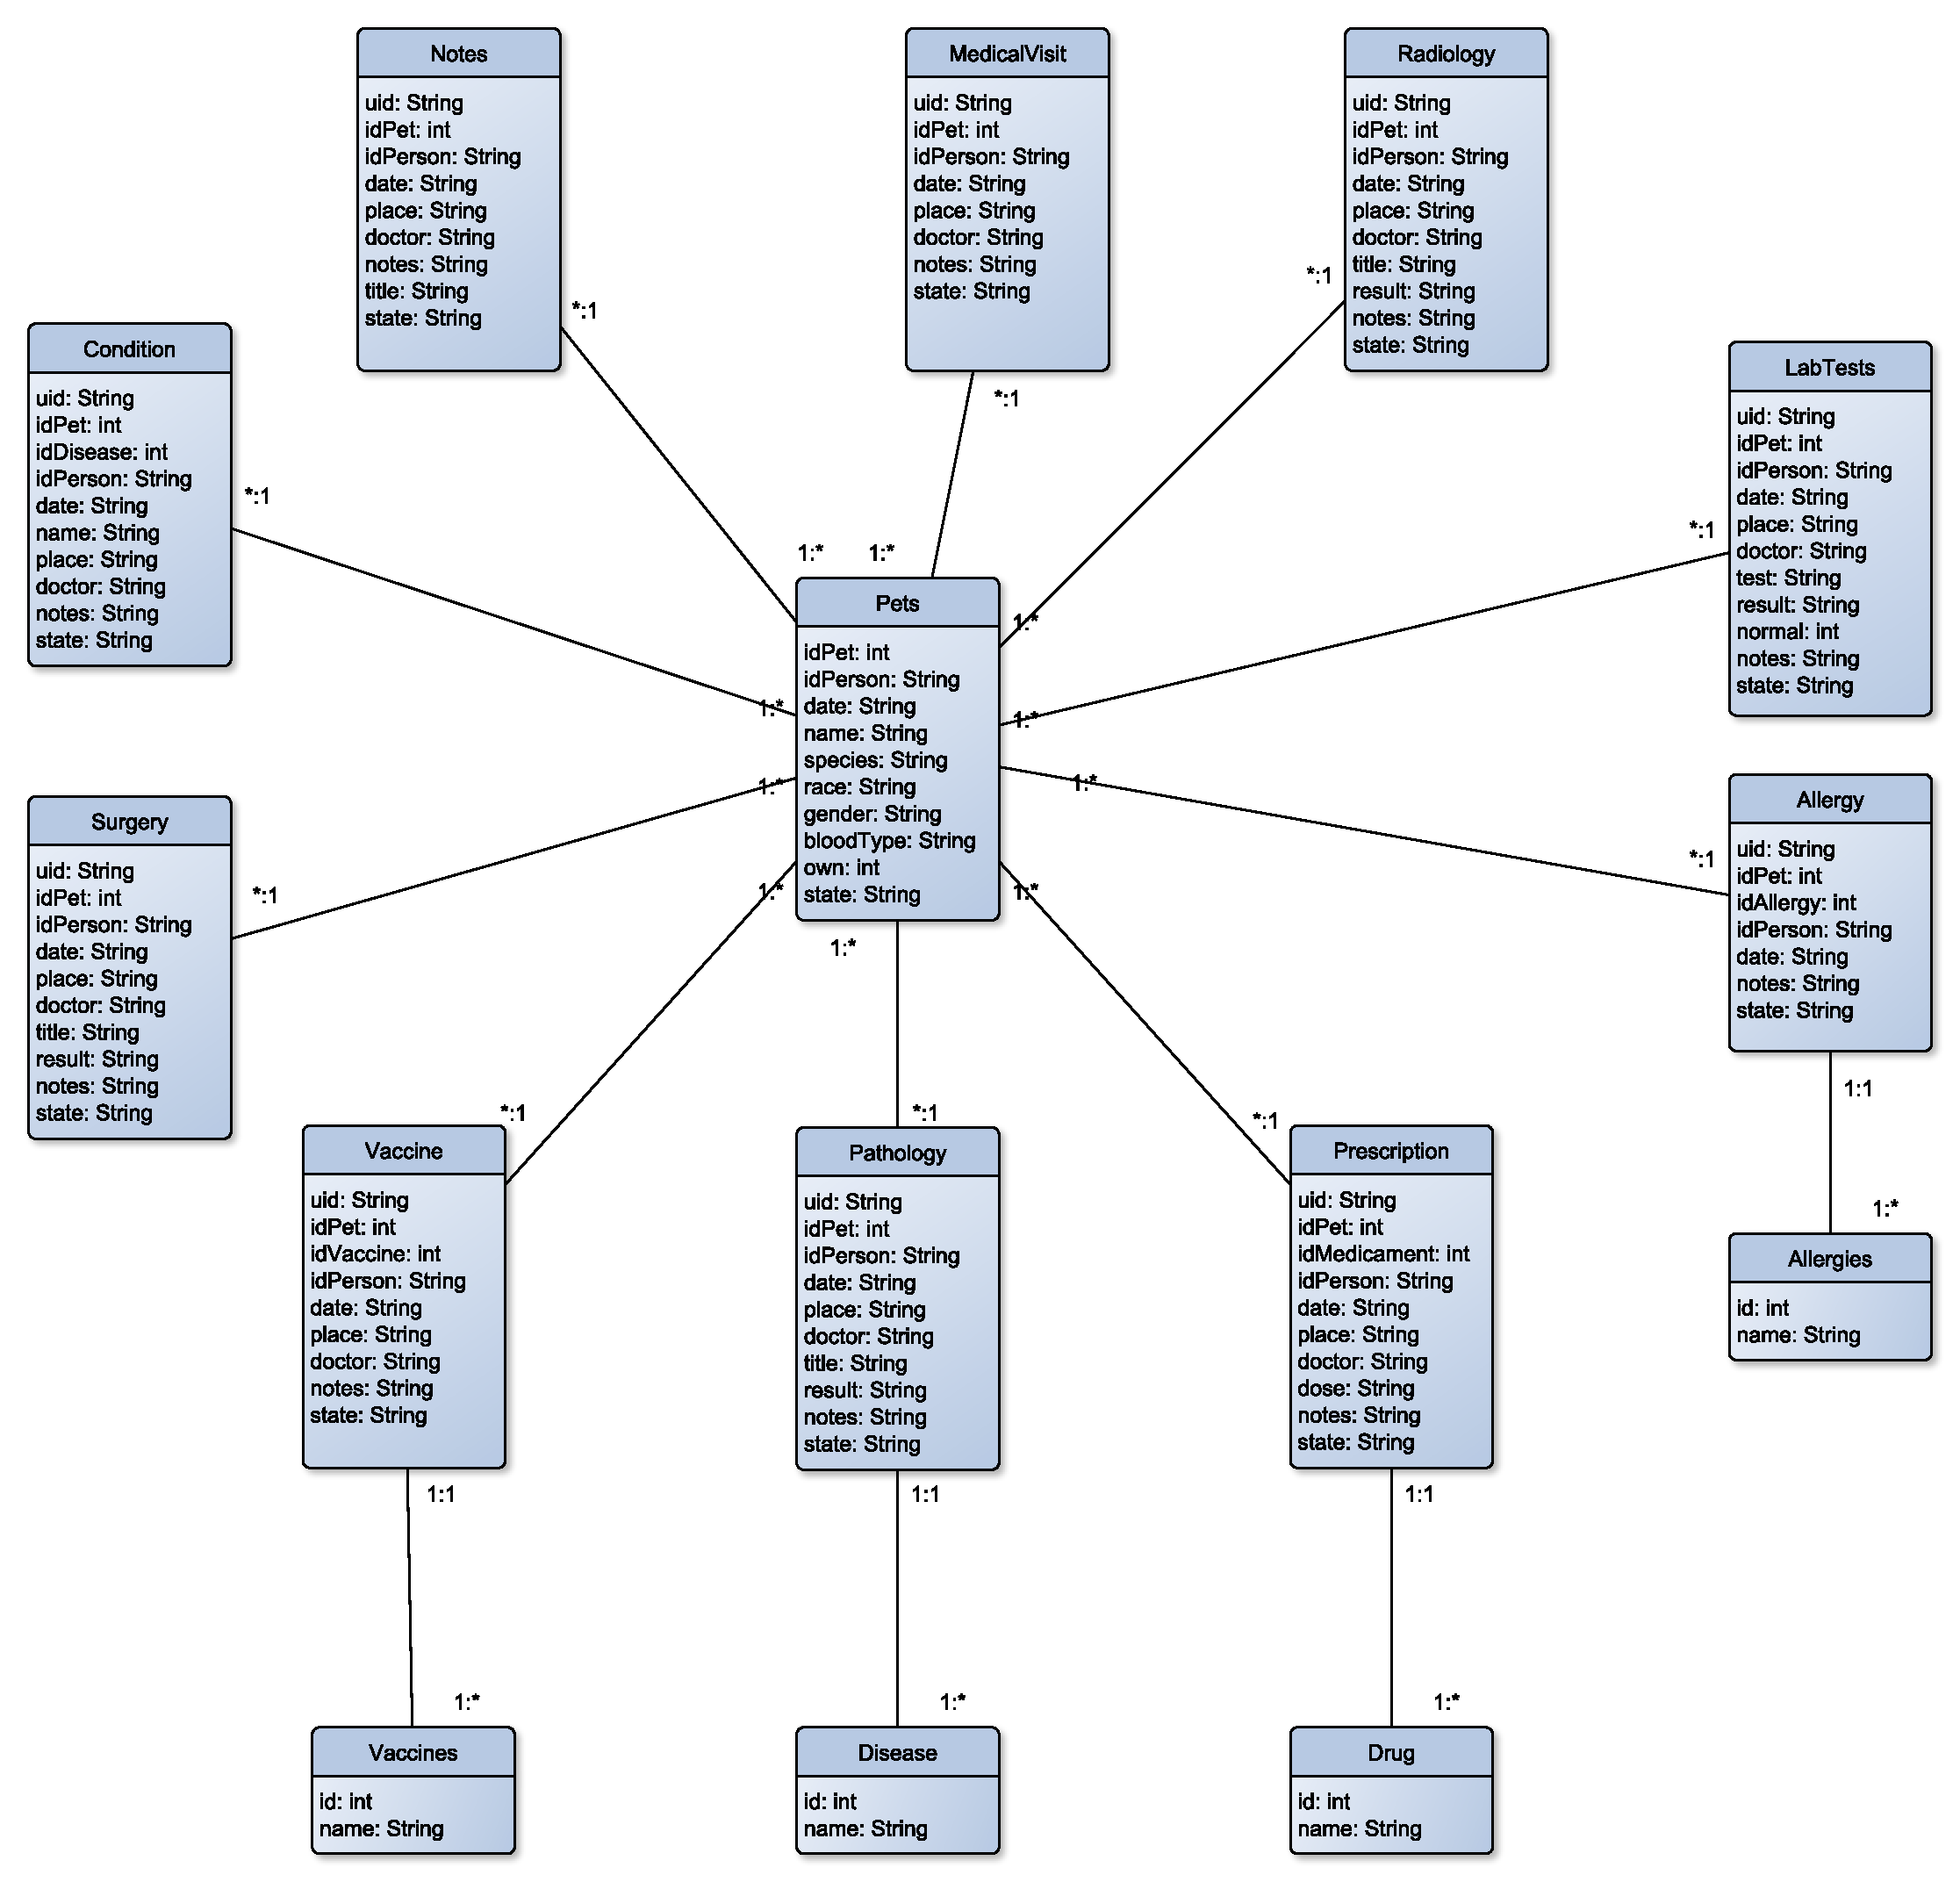
\includegraphics[scale=0.3]{Graphics/model1.pdf}
\caption{Representación del modelo de la base de datos}
\label{fig:rcm}

\end{center}
\end{figure}




Para la creación y acceso a la clase DatabaseHandler; clase encargada de manejar las solicitudes a la base de datos en nuestra aplicación, se utilizó como patrón de diseño singleton. 

\textbf{Singleton} \brackcite{single} es un patrón de diseño creacional que consiste en tener durante toda la ejecución de un programa sólo una única instancia de una clase dada; proveyendo además un punto de acceso global a dicha instancia. Esto se logra entre otras cosas haciendo privado el método constructor de la clase y ofreciendo acceso a esta a través de un método especial de tipo get. Dicho método es el encargado de verificar si existe creada una instancia de esa clase y devolverla o crearla dependiendo del caso. De esta forma se asegura la propia clase de haber sido creada una única vez y por tanto tener una única instancia (singleton).



\chapter{Detalles de Implementación}
\label{chapter:implementation}


\section{Tecnologías utilizadas en HCVet}


\subsection{Dart}


\begin{figure}[h!]
\begin{center}

\includegraphics[scale=0.4]{Graphics/images/LogoDart.png}
\caption{Logo de Dart}
\label{fig:rcm}

\end{center}
\end{figure}

Para la implementación de la aplicación se empleó como núcleo principal $Dart$ \brackcite{dart}. $Dart$ es un lenguaje optimizado para el desarrollo rápido de aplicaciones en cualquier plataforma, su objetivo es ofrecer el lenguaje de programación más productivo para el desarrollo multiplataforma. $Dart$ es un lenguaje orientado a objetos, basado en clases, con una sintaxis similar a $C$ y con $Garbage Collector$\footnote{Garbage Collector o Recolector de basura es un mecanismo implícito de gestión de memoria implementado en algunos lenguajes de programación de tipo interpretado o semi-interpretado.}. Admite interfaces, genericidad\footnote{Es una propiedad que permite definir una clase o función sin especificar el tipo de datos de uno o mas de sus parámetros }, mixins\footnote{Es una clase que contiene métodos para ser usados por otras clases sin tener que ser la clase padre de esas otras clases. }, clases abstractas,  e inferencia de tipos. 

$Dart$ también es la fundación de $Flutter$ proveyendo el lenguaje y los tiempos de ejecución que caracterizan a $Flutter$.

%https://dart.dev/overview


\subsection{Kotlin}

\begin{figure}[h!]
\begin{center}

\includegraphics[scale=0.11]{Graphics/images/LogoKotlin.jpg}
\caption{Logo de Kotlin}
\label{fig:rcm}

\end{center}
\end{figure}

Para la implementación de algunas funcionalidades de la aplicación se utilizó $Kotlin$ \brackcite{kot}. $Kotlin$ es el lenguaje oficial para desarrollo de aplicaciones en $Android$ declarado por $Google$ en el $2019$. $Kotlin$ es un lenguaje de programación multiplataforma que remueve detalles superfluos de $java$ como $null pointer exceptions$ \footnote{$null pointer exceptions$ es una excepción que ocurre cuando una variable es accedida en ejecución y esta no está apuntando a ningún objeto} y es un lenguaje más simple y práctico en comparación con $java$.




%https://developer.android.com/kotlin/overview
\subsection{Paquete http}

\textbf{http} es una biblioteca de $Flutter$ basada en \textbf{Future}\footnote{Una instancia de la clase \textbf{Future} representa el resultado de una operación asíncrona} para hacer \textbf{requests} de $HTTP$.

Esta biblioteca es multiplataforma que permite su uso en dispositivos de escrito, dispositivos móviles y en navegadores web. Contiene una variedad de funciones y clases de alto nivel que facilitan el consumo de recursos $HTTP$. 

\textbf{http} \brackcite{httpF} es uno de los paquetes más aclamados de $Flutter$ que se encuentran disponible en $pub.dev$.

\subsection{Paquete uuid}
Este complemento para $Flutter$ se encarga del análisis y la generación simple y rápida de \textbf{UUID}\footnote{Identificador Único Universal}  RFC4122. Entre las posibles opciones de obtención de uuid la que se utilizó para las llaves de las tablas fue la basada en el tiempo \brackcite{uuid}. 


\subsection{Paquete encrypt}
Esta biblioteca contiene un conjunto de APIs de alto nivel sobre $PointyCastle$\footnote{$PointyCastle$ es una biblioteca de $Dart$ para encriptación y desencriptación.} para criptografía simétrica. Facilita la generación de llaves aleatorias seguras y Vectores de Inicialización.


\subsection{Paquete sqfentity}
\textbf{SQLite}\brackcite{sqli} es una biblioteca en lenguaje $C$ que implementa un motor de base de datos $SQL$ pequeño, rápido, autónomo, de alta confiabilidad y con todas las funciones. El formato de archivo que utiliza es estable, multiplataforma y compatible con versiones anteriores.
 
Entonces llegamos a \textbf{sqfentity}\brackcite{sqfen}, un $ORM$\footnote{Es una técnica de programación para convertir datos entre el sistema de tipos utilizado en un lenguaje de programación orientado a objetos y la utilización de una base de datos relacional como motor de persistencia.}  para $Flutter$ $SQLite$. Se basa en el paquete $sqflite$, para la misma plataforma, permitiendo compilar y ejecutar comandos $SQL$ de manera fácil y rápida con la ayuda de métodos fluidos similares a $.Net Entity Framework$\footnote{Es un moderno ORM para .Net.}.

\section{Detalles de la Implementación}
\label{chapter:implementation}

\subsection{Estructura de Model}

En el Modelo de la aplicación se buscó proporcionar todas funcionalidades deseadas del producto de la forma más legible y escalable a futuro que fuera posible. Con este objetivo los autores tomaron el patrón de arquitectura de micro-servicios \brackcite{arqPat}, se dividió el modelo en 3 componentes de servicio: 

\begin{itemize}
\item Componente de comunicación con el servidor ($Online$)
\item Componente de comunicación con otro dispositivo ($Offline$)
\item Componente de almacenamiento interno ($Database$)
\end{itemize}

Con los componentes de servicio definidos se emplean las interfaces del $ViewModel$ para acceder a estos servicios. Consideramos que este diseño permitía crear un modelo escalable horizontalmente además de facilitar el mantenimiento y actualización de dichos componentes.

\subsection{Implementación del componente Offline}

Uno de los requerimientos fundamentales del producto era lograr la compatibilidad con la mayor cantidad de dispositivos móviles que fuera posible, intentando evitar la necesidad de adquirir un dispositivo móvil moderno para poder utilizar el producto.

Durante la investigación realizada para satisfacer este requisito los autores encontraron un problema: los paquetes de $Flutter$ encontrados que permiten el manejo las conexiones entre dispositivos a través de $Wifi$ restringían el uso de diferentes $APIs$ como la creación de $Hotspots$ locales para $Kit$ de Desarrollo de Software ($SDK$)\footnote{Un $kit$ de desarrollo de software ($SDK$) es un conjunto de herramientas proporcionado usualmente por el fabricante de una plataforma de $hardware$, un sistema operativo o un lenguaje de programación.} de $Android$ mayor o igual que $26$ \footnote{$Android$ $SDK$ $26$ refiere al sistema operativo $Android$ $8.0$} \brackcite{wifiIOT}.

Para suplir esta necesidad se utilizo el $API$ $WifiP2pManager$ de $Android$. Esta $API$ permite a la aplicación descubrir $peers$\footnote{$peer$ es cualquier usuario que se conecta a la red de intercambio} disponibles y permite establecer una conexión directa con estos. Usando $Kotlin$ se definió el comportamiento de los $peers$ y se creó una interfaz para acceder a las funcionalidades de esta $API$.

\subsubsection{¿Cómo se usa esta interfaz desde $Flutter$?}


$Flutter$ permite realizar llamados a $APIs$ específicas de la plataforma disponibles en $Java$ o $Kotlin$ en $Android$ y en $Objective$ $C$ o $Swift$ en $iOS$

Desde la aplicación de $Flutter$ se envía un mensaje a un $host$ en $Android$ o $iOS$ a través de un canal entre plataformas. Tanto el mensaje como la respuesta se pasan de forma asíncrona.

\subsection{Implementación del componente Online}
La comunicación con el servidor está basada en un protocolo de tipo $Hypertext$ $transfer$ $protocol$ $secure$ ($HTTPS$) de $request-response$. Se consideró la encriptación de los datos en ambas direcciones que ofrece el protocolo $https$ para evitar la vulneración de datos sensibles transferidos como pueden ser el $id$ del usuario o la mascota, correo y contraseña.

\subsection{Sincronización de la base de datos local con el servidor}
Dentro de las problemáticas encontradas durante el proceso de sincronización de la base de datos local con la del servidor se pudieran mencionar las siguientes:
\begin{enumerate}

\item\textbf{Diferenciar los datos}: en cualquier momento dado en la base de datos local existirán datos que ya el servidor tendrá conocimiento de ellos y por tanto se puede decir que están sincronizados con el servidor y otros datos de nueva creación que hasta que no exista una conexión a internet, el servidor desconocerá por completo de su existencia y por tanto estarán pendientes a sincronizar. Diferenciar cuales de estos datos ya están sincronizados y cuales no, resulta un poco complejo de manejar si no se utiliza algún mecanismo de “control” sobre ellos. Todo esto para intentar reducir el número de envío de información al servidor por cuestiones de seguridad y rapidez, puesto que bien se podrían enviar todos los datos de la base de datos local al servidor cada vez que exista una conexión, pero esta opción además de no factible resulta lamentable. Para solucionar dicha problemática se optó por agregar en cada tabla de la base de datos un campo extra llamado “$state$”. Dicho campo tendrá el valor “$waiting$” cuando es un dato nuevo y el valor “$synchro$” cuando ya ha sido sincronizado con el servidor. Cuando los datos son creados desde el propio teléfono la función de insertar elementos en la base de datos declara el campo $state$ de dicho objeto como $waiting$, sin embargo, cuando los datos provienen de otro móvil o incluso del propio servidor se declara el $state$ como $synchro$ puesto que no es necesario re sincronizar  estos datos.
\item\textbf{Guardar llaves de futuras mascotas}: cuando el usuario se registra en el servidor y/o realiza algún tipo de suscripción, el servidor manda una lista de futuras llaves para la creación de nuevas mascotas. Para no tener que implementar una nueva tabla que tan solo guardase estas llaves o bien almacenarlas en un fichero apartado de la base de datos, se optó por almacenar en la tabla $Pets$ una mascota “vacía”. Dicha mascota tendrá en sus campos solo esta llave como llave primaria y el $state$ tendrá el valor “$empty$” indicando de este modo que la mascota aun no existe en la base de datos. Cuando se crea una nueva mascota que tiene alguna de estas llaves como llave primaria se actualizan los campos de la mascota ya “previamente” insertada en la base de datos y su $state$ cambia a “$waiting$”.
\item\textbf{Guardar mascotas eliminadas}: aunque pareciese una contradicción hay momentos en la que nuestra base de datos necesita mantener guardada aun una mascota que ha sido eliminada por el usuario. Como nuestra base de datos debe ser sincronizada con la existente en el servidor no basta con eliminar una mascota directamente de la base de datos cuando el usuario requiera esta operación puesto que, si la mascota deja de existir, luego cuando exista una conexión a internet no habrá manera de indicar al servidor que debe eliminar dicha mascota de su base de datos también. Para resolver esta problemática se hace uso nuevamente del campo $state$ en mascota. Cuando el usuario manda a eliminar una mascota de la aplicación, se actualiza el $state$ de dicha mascota a valor “$delete$” indicando así al resto de los métodos de la base de datos que esa mascota, aunque está insertada no cuenta como una mascota válida (este funcionamiento se extiende también a todas las tablas que tienen como llave foránea un id de dicha mascota). Luego de que se indique al servidor que debe eliminar dicha mascota se eliminará también de la base de datos local.
\end{enumerate}

\chapter{Pruebas de Funcionalidad y Experimentos}

En este capítulo se realizan un conjunto de pruebas para demostrar el funcionamiento de las herramientas implementadas en la aplicación.

Las pruebas fueron realizadas en dos teléfonos $android$ con las siguientes características.

Primer teléfono:

\begin{itemize}
\item Procesador: Hisilicon Kirin $710F$.
\item 4 $GB$ de $RAM$.
\item Sistema Operativo Android $9$
\end{itemize} 

Segundo teléfono:

\begin{itemize}
\item Procesador: Octa-core Max $2.00GHz$.
\item 4 $GB$ de $RAM$.
\item Sistema Operativo Android $12$
\end{itemize} 

\newpage
\section{Prueba 1: Creación de cuenta o autentificación de usuario}

\begin{figure}[h!]
\begin{center}

\includegraphics[scale=0.25]{Graphics/images/hcvet/init.jpg}
\caption{De izquierda a derecha: Página inicial de la aplicación, página de creacióm de usuario y página de autentificación}
\label{fig:bac}

\end{center}
\end{figure}

Se requiere que el usuario introduzca un nombre de usuario y contraseña para crear una cuenta en el servidor. La aplicación también utiliza el número de teléfono del dispositivo para identificar al usuario. En caso de que el número de teléfono o el correo introducido ya se encuentre registrado la aplicación muestra un error y espera una corrección por parte del usuario.

\newpage
 
\section{Prueba 2: Creación de mascota}

\begin{figure}[h!]
\begin{center}
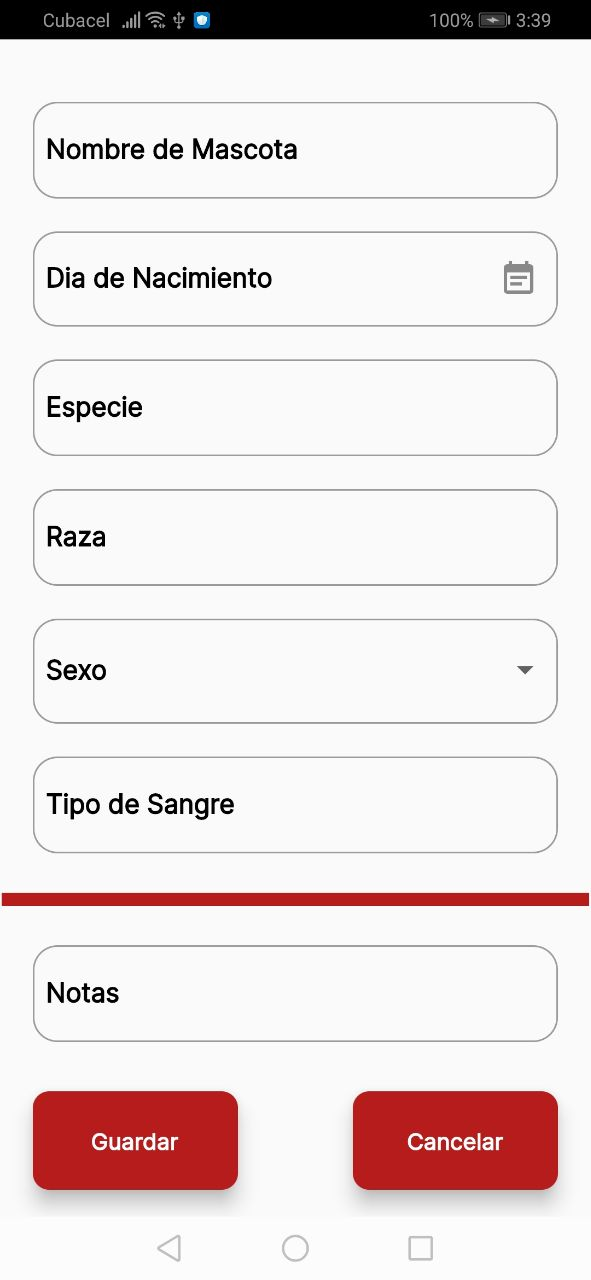
\includegraphics[scale=0.15]{Graphics/images/hcvet/addpet.jpg}
\caption{ Página de creación de mascotas}
\label{fig:bac}

\end{center}
\end{figure}

La creación de una mascota requiere que el usuario introduzca todos los campos que se listan a excepción de $notas$. Solo se permite la creación de una mascota si el usuario tiene un $id$ disponible en la base de datos local.

\begin{figure}[h!]
\begin{center}
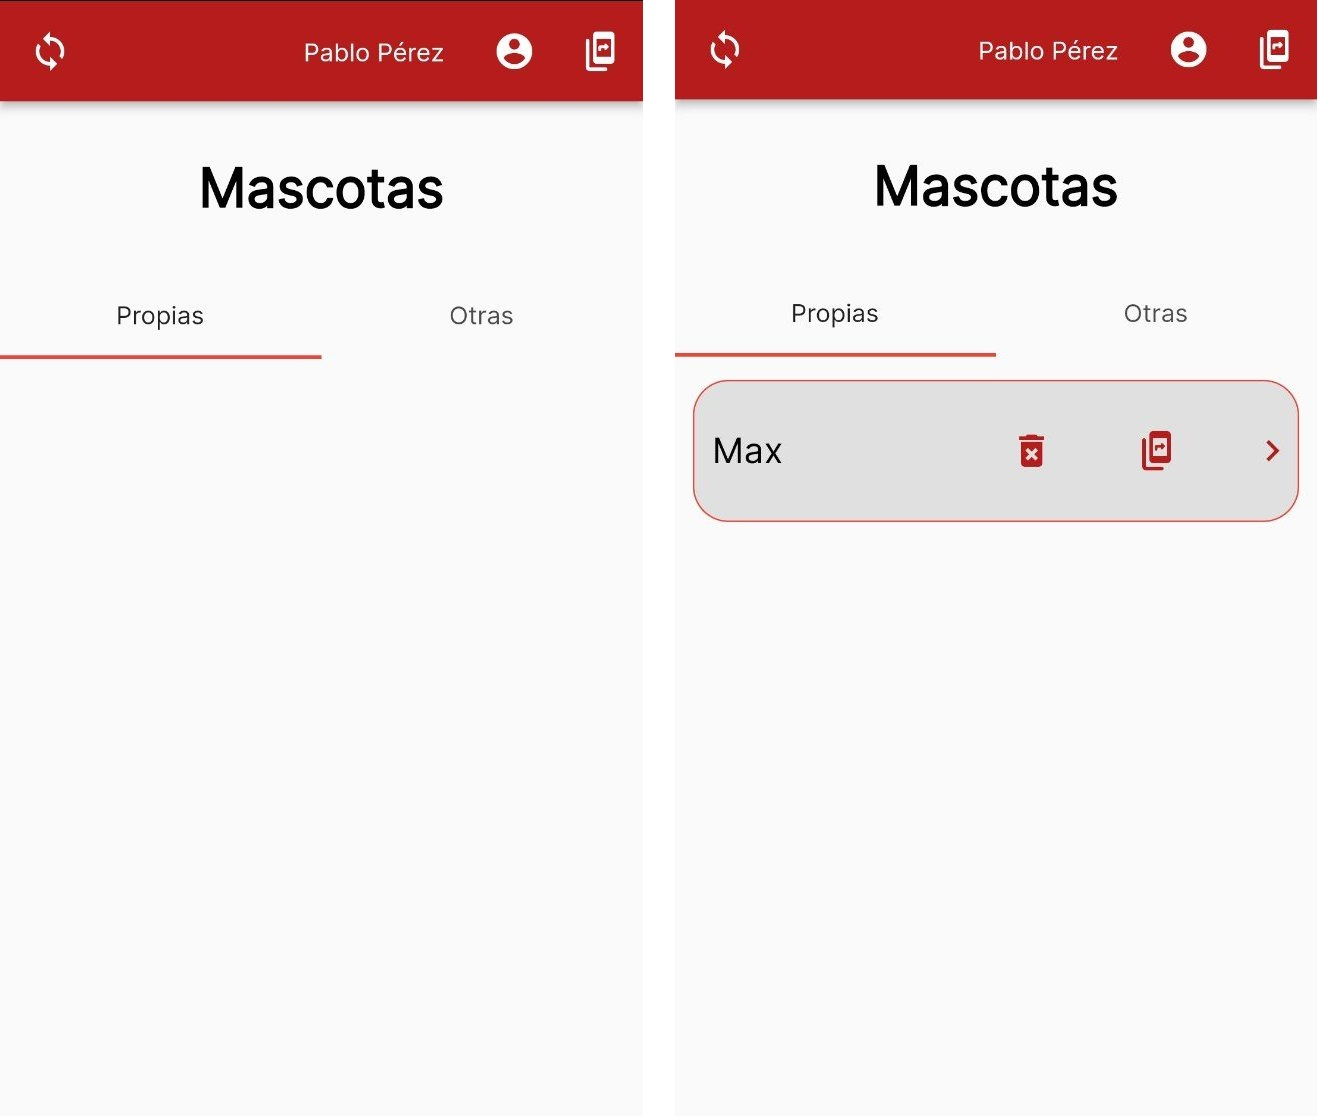
\includegraphics[scale=0.19]{Graphics/images/hcvet/home.jpg}
\caption{ Página de central de la aplicación antes y después de crear una mascota}
\label{fig:bac}

\end{center}
\end{figure}

Página central de la aplicación antes y después de crear una mascota

\newpage
\section{Prueba 3: Eliminar mascota}

\begin{figure}[h!]
\begin{center}
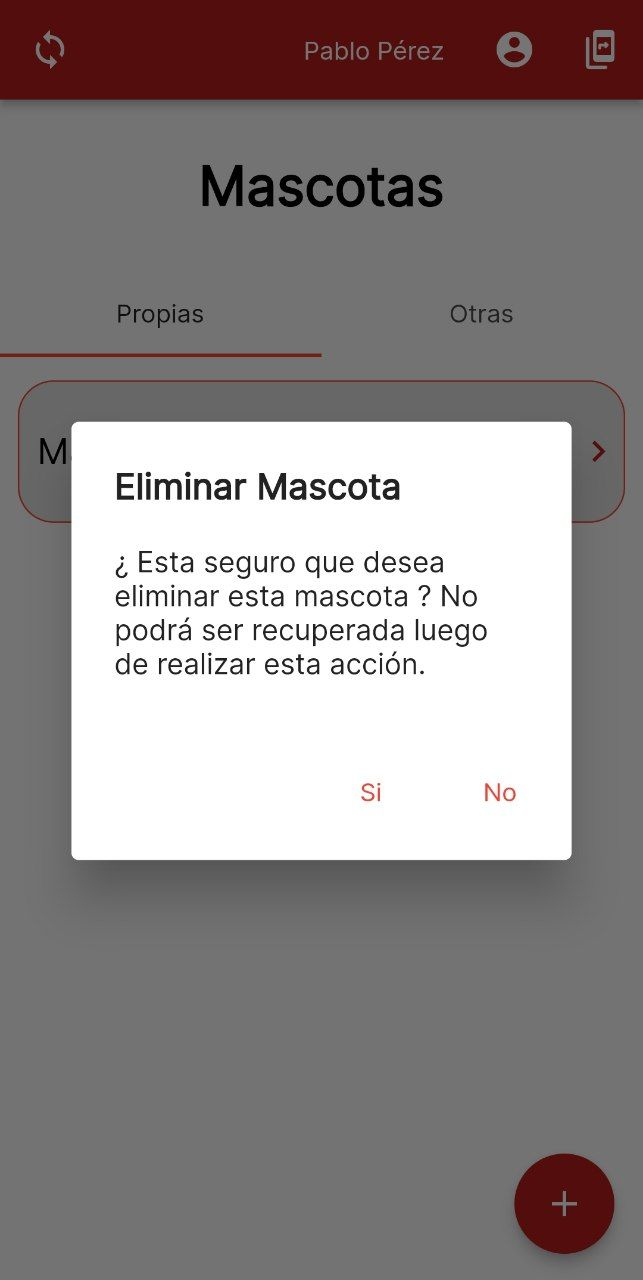
\includegraphics[scale=0.19]{Graphics/images/hcvet/delete.jpg}
\caption{ Advertencia al eliminar una mascota}
\label{fig:bac}

\end{center}
\end{figure}

Si el usuario decide eliminar una mascota los datos e historial de consultas de estas no podrán ser recuperados. Esta advertencia es mostrada ante el usuario, si escoge eliminar la mascota el servidor será notificado de esta decisión la próxima vez que se sincronice.


\newpage

\section{Prueba 4: Creación y mostrado de consultas}


\begin{figure}[h!]
\begin{center}
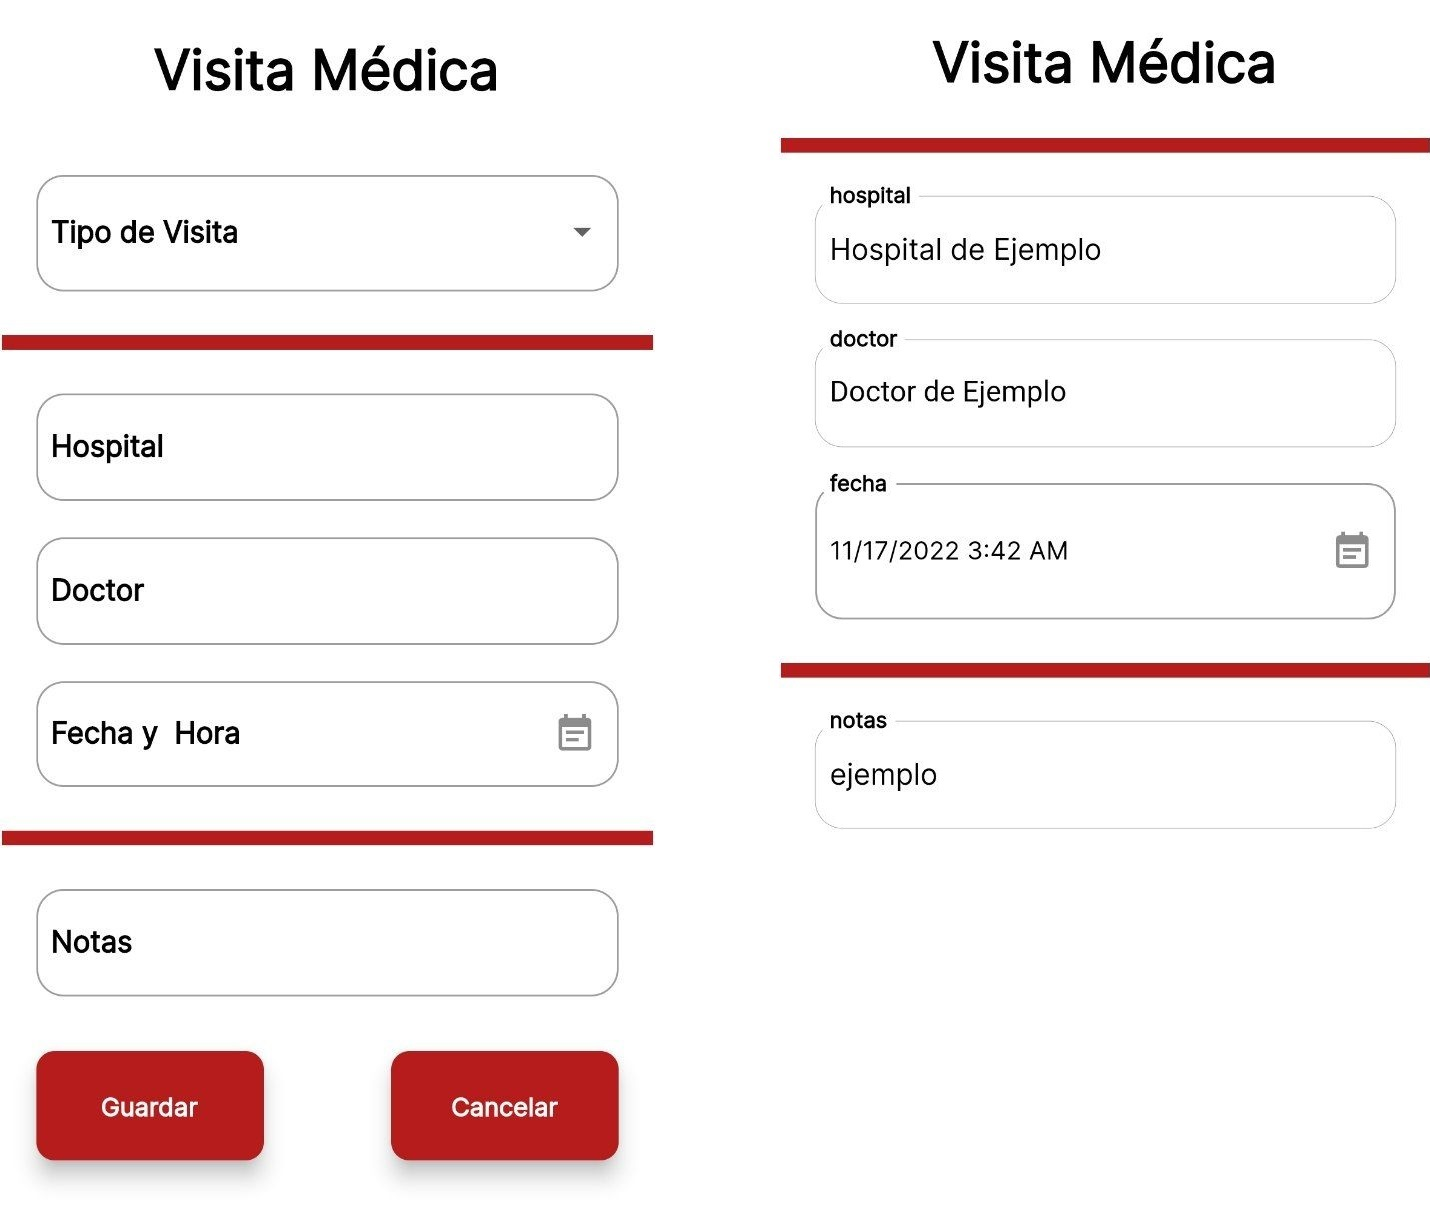
\includegraphics[scale=0.15]{Graphics/images/hcvet/medvisit.jpg}
\caption{Página de creación de consulta Visita Médica y página de mostrado de esta consulta}
\label{fig:bac}

\end{center}
\end{figure}

La creación de una consulta solo requiere un dato fundamental, la fecha. Las consultas de Prescripción, Vacuna, Condición y Alergia requieren que se seleccione una de las llaves foráneas de la respectiva consulta. El usuario es notificado si uno de estos requerimientos no se cumple.

\begin{figure}[h!]
\begin{center}
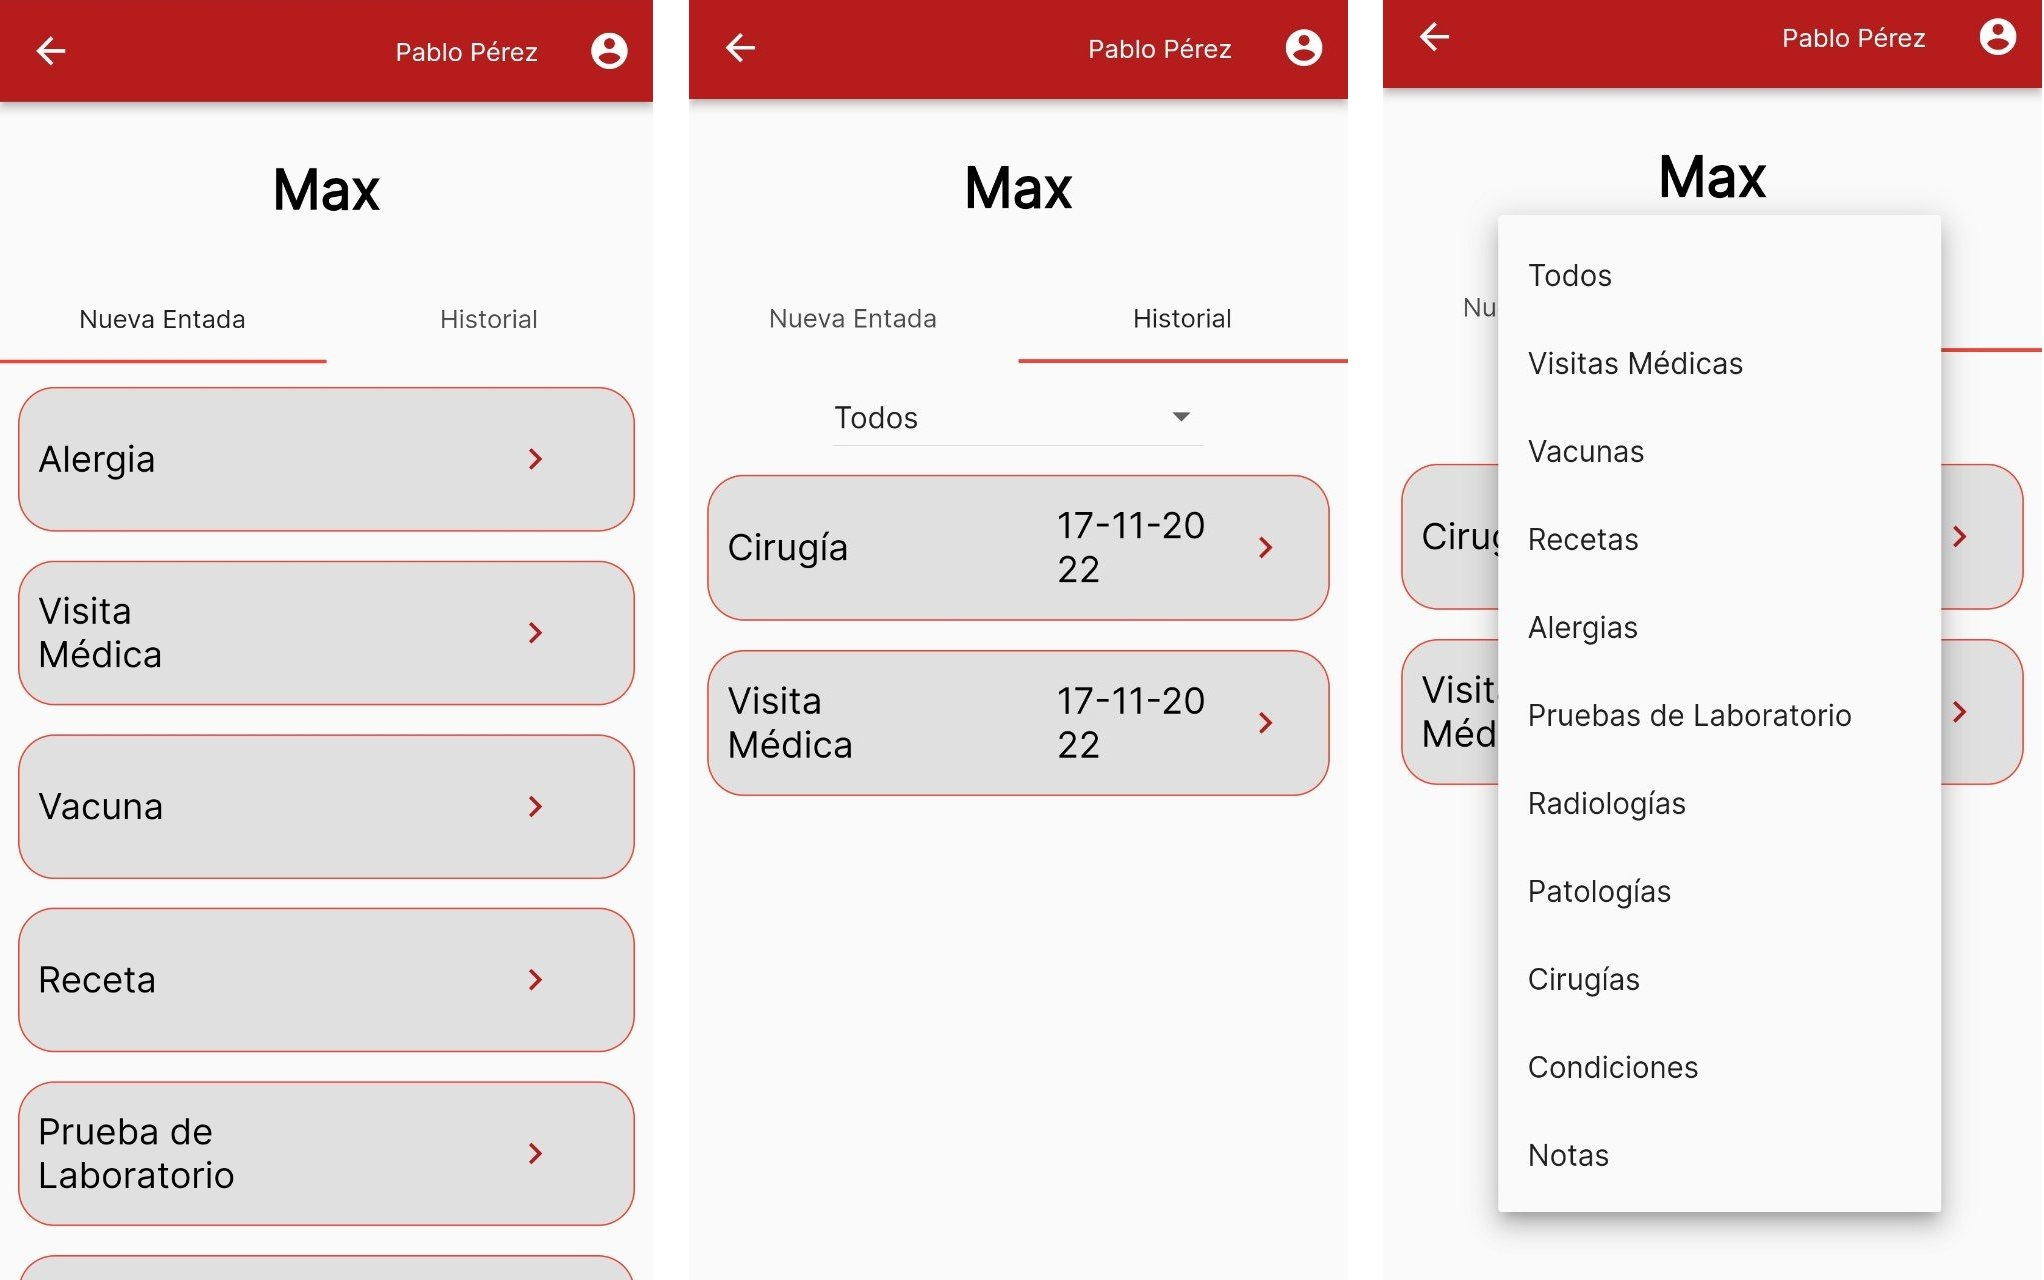
\includegraphics[scale=0.17]{Graphics/images/hcvet/formsmake.jpg}
\label{fig:bac}
\caption{De izquierda a derecha: Página de selección de consulta a agregar, historial de consultas y filtrado de consultas en historial}
\end{center}
\end{figure}

Con una mascota seleccionada se dirige al usuario a la página de manejo de consultas, el usuario puede crear una consulta nueva o acceder a todas las consultas que se encuentran almacenadas en la base de datos local.
\backmatter
\chapter*{Conclusiones}\label{chapter:conclusions}

Controlar la información medica de una mascota es un tema de suma importancia, que es llevado a cabo en su mayoría de manera poca eficiente y raramente digital. Durante el proceso investigativo que los autores emplearon en la realización de este trabajo de diploma, encontraron clara la necesidad de la existencia de un programa que permitiera el almacenamiento, organización y distribución de datos en el sector veterinario. Con el desarrollo de HCVet, se le dio cumplimiento a los objetivos trazados en el capítulo 1. La aplicación construida es capaz de mostrar información contenida en la historia clínica veterinaria de las mascotas del usuario sin necesidad de una conexión a Internet, así como añadir nueva información por medio de formularios construidos de forma dinámica a partir de distintas categorías. Siendo también posible compartir información entre usuarios utilizando la wifi. En este trabajo, se muestra el diseño de la base de datos utilizada, y algunos de los problemas surgidos durante la implementación, así como los mecanismos utilizados para dar solución a estas problemáticas. La aplicación desarrollada muestra un gran potencial que soluciona no solo los problemas planteados, sino la habilidad para expandirse a otros campos u objetivos. 
\begin{opinion}
    Opiniones de los tutores
\end{opinion}
\begin{recomendations}
    Aunque consideramos que HCVet cumple con todas las características y funcionalidades propuestas no debe descartarse la opción de que en futuras versiones de la aplicación se incorporen nuevas funcionalidades que no contemplamos en esta versión actual. Entre algunas de las posibles acciones a realizar en un futuro con el objetivo de ampliar los casos de uso de la aplicación se proponen las siguientes ideas:

\begin{enumerate}


\item Investigar sobre otros tipos de consultas que pudieran ser añadidas al modelo de la aplicación.

\item Diferenciar entre distintos tipos de usuarios (dueño, veterinario, estilista, etc.) y establecer cuáles serían sus permisos sobre los datos de la aplicación.

\item Añadir la opción de modificar los datos de una mascota y/o los de una consulta previamente existente.

\item Implementar un sistema de citas controlado por el servidor para que los médicos veterinarios tengan un espacio para coordinar las consultas con los clientes.

\item Implementar un sistema de avisos y alarmas que indiquen al usuario sobre las visitas pre-programadas al veterinario y/o el horario de darle una medicina a su mascota.
\end{enumerate}
\end{recomendations}

\printbibliography[heading=bibintoc]



\end{document}